\section{Results and Discussion}

\subsection{HPCC}

As already mentioned before, the \texttt{hpcc} test consists in a large number of benchmarks; the full resoults can be found in the folder \href{https://github.com/giovanni-lucarelli/cloud-basic/tree/main/results}{results} in the github repository of the project. For clarity sake here are reported and discussed only the principal ones, divided according to the hardware stressed.

\subsubsection{Compute Performance}

This section evaluates the computational performance of the system across different environments. Specifically, the benchmark reported are: HPL (High-Performance Linpack), DGEMM (Double-precision General Matrix Multiply), and FFT (Fast Fourier Transform). All of them aim to assess floating-point computation in linear algebra and numerical problems. As presented in Table \ref{tab:benchmark_performance} and in Figure \ref{fig:hpcc_compute_performance}, the results consistently show that the container environment performs comparably to or exceeds the host environment across most metrics, while the virtual machine (VM) configuration trails behind.

A notable observation is the significant performance disparity exhibited by the VMs in the MPI FFT benchmark. Parallel FFT algorithms are inherently communication-intensive, frequently requiring extensive inter-rank communication, typically involving all-to-all exchanges for data transposition and redistribution. Consequently, beyond raw floating-point capability, this workload heavily stresses: network latency and bandwidth and MPI transport efficiency. A critical distinction among the three environments lies in their respective MPI communication mechanisms. On the host system, MPI communication between processes on the same node primarily utilizes highly efficient shared memory. In contrast, the container environment employs the TCP network protocol for inter-process communication, albeit potentially with lower overhead compared to VMs due to reduced virtualization layers. The VM environment, however, relies on TCP communication routed through virtual Network Interface Controllers (vNICs). This virtualization layer for networking introduces substantial overhead, resulting in significantly poorer latency and bandwidth characteristics for inter-process communication within and between VMs. These detrimental effects of virtualized networking on communication performance are clearly corroborated by the results of the ping-pong and iperf network benchmarks, presented in Table \ref{tab:pingpong} and Table \ref{tab:iperf}, respectively, which demonstrate substantially higher latency and lower bandwidth for the VM environment.

\begin{table}[htbp]
\centering

\renewcommand{\arraystretch}{1.2}
\begin{tabular}{lccc}
\toprule
\textbf{Benchmark} & \textbf{VM} & \textbf{Container} & \textbf{Host} \\
\midrule
\textbf{HPL (Gflops)} & 5.128 ± 0.013 & 5.552 ± 0.034 & 5.516 ± 0.027 \\
\midrule
\textbf{DGEMM (Gflops)} & & & \\
StarDGEMM     & 1.290 ± 0.045 & 1.303 ± 0.122 & 1.400 ± 0.005 \\
SingleDGEMM   & 1.907 ± 0.077 & 2.081 ± 0.052 & 2.054 ± 0.024 \\
\midrule
\textbf{FFT (Gflops)} & & & \\
StarFFT      & 1.453 ± 0.033 & 1.832 ± 0.025 & 1.816 ± 0.008 \\
SingleFFT    & 2.638 ± 0.047 & 2.767 ± 0.054 & 2.739 ± 0.141 \\
MPIFFT       & 1.231 ± 0.064 & 3.673 ± 0.124 & 4.042 ± 0.014 \\
\bottomrule
\end{tabular}
\caption{Benchmark performance (in Gflops) across the three execution environments. Values are reported as mean ± standard deviation, calculated over three measurements ($n = 3$).}
\label{tab:benchmark_performance}
\end{table}

\begin{figure}[htbp]
    \centering
    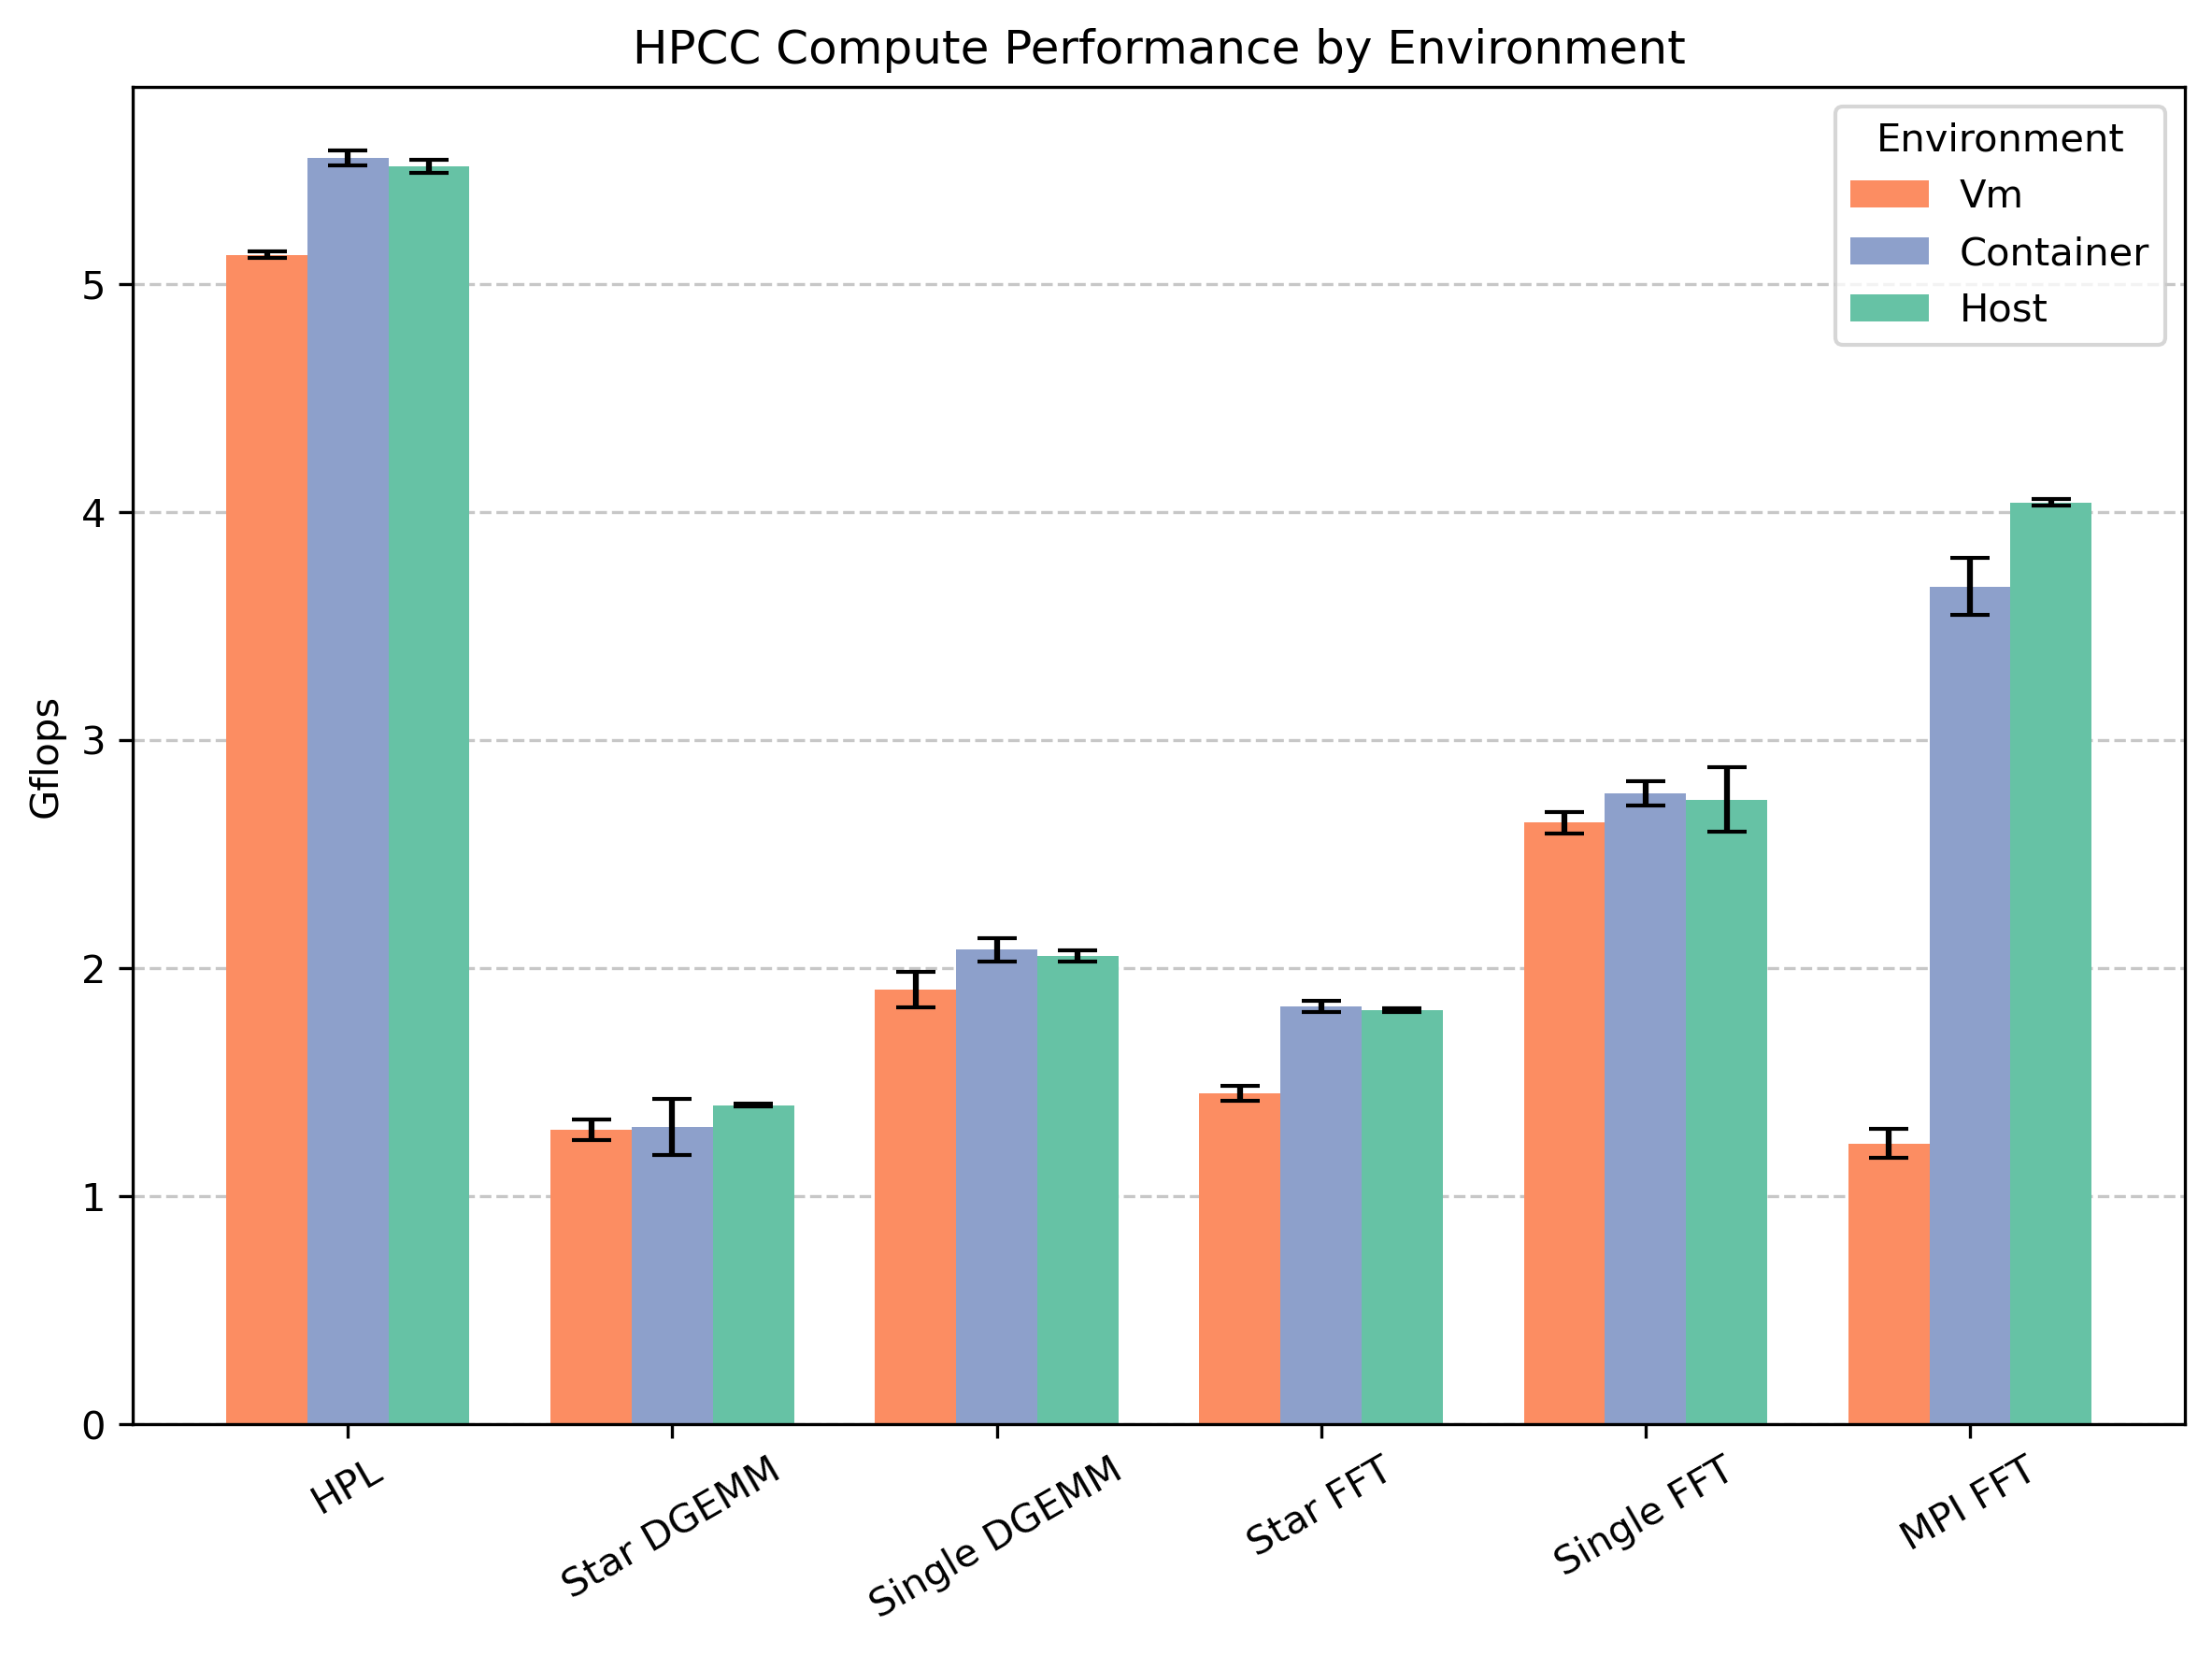
\includegraphics[width=0.8\linewidth]{assets/hpcc_compute_performance.png}
    \caption{Compute Performance Benchmarks: VM (orange) vs Container (blue) vs Host (green). All the benchmarks are reported in Gflops.}
    \label{fig:hpcc_compute_performance}
\end{figure}

\subsubsection{Memory Benchmarks}
The main memory benchmark results are presented in Table \ref{tab:memory_performance_hpcc} and Figure \ref{fig:hpcc_memory_performance}. The benchmarks include SingleSTREAM, StarSTREAM, RandomAccess, and PTRANS. Each benchmark is designed to evaluate different aspects of memory performance, including bandwidth and latency.

\paragraph{STREAM Memory Bandwidth}

The STREAM benchmark measures sustainable memory bandwidth (typically reported in GB/s) through simple vector operations: \textit{Copy}, \textit{Scale}, \textit{Add}, and \textit{Triad}. The benchmark was executed in two configurations: SingleSTREAM, assessing memory performance on a single compute node, and StarSTREAM, which aggregates memory bandwidth across multiple nodes in a distributed setting.

In SingleSTREAM evaluations, the host and container environments demonstrated comparable memory bandwidth, while the virtual machine (VM) configuration consistently exhibited lower performance. Despite the VM's relative underperformance, all environments achieved a substantial percentage of the theoretical maximum bandwidth, indicating generally efficient operation of the local memory subsystems, with the exception of the VM, which is subject to certain virtualization-induced memory overheads.

To determine the nominal memory bandwidth of the system, hardware information was queried using the command \texttt{sudo dmidecode --type memory}. The relevant output is presented below:

\begin{minted}{text}
Configured Memory Speed: 1867 MT/s
Bus width per channel: 64 bits = 8 bytes
Number of channels: 2
\end{minted}

Based on this information, the theoretical peak memory bandwidth can be calculated as follows:

\begin{equation*}
\text{Bandwidth} = 1.867 \frac{\text{GT}}{\text{s}} \times 8 \frac{\text{B}}{\text{T}} \times 2 = 29.872 \frac{\text{GB}}{\text{s}}
\end{equation*}

Among the STREAM operations, the \textit{Copy} operation -- being highly optimized by compilers and frequently implemented using assembly code -- provides the most direct measure of effective memory throughput. The observed throughput for the \textit{Copy} operation was approximately 75\% of the nominal bandwidth for the VM, 81\% for the container, and 78\% for the host. These results indicate generally satisfactory performance across all environments.

In the \textbf{StarSTREAM} benchmark the container environment again surpassed the VM setup. As data exchange between nodes necessitates significant network communication and synchronization, the effective memory bandwidth becomes constrained also by network bandwidth and latency rather than only local memory speed. Consequently, performance declines significantly compared to SingleSTREAM, with the observed bandwidth reaching only approximately 20\% of the nominal maximum. This performance degradation is particularly pronounced in the VM cluster, probably due to the overhead associated with the virtualized of the network interface.

\paragraph{RandomAccess (RA) Benchmark}

The RandomAccess benchmark quantifies the rate of random memory updates, expressed in mega updates per second (MUP/s). Unlike STREAM, which focuses on sequential memory access patterns, RandomAccess evaluates the system's efficiency in handling numerous small, non-contiguous memory accesses. 

In the MPI implementation of this benchmark, the host environment exhibited disproportionately high performance. This can be interpreted analogously to the case of MPI FFT and so can be attributed to the utilization of shared memory for inter-process communication on the host, which is substantially more efficient than the network-based communication employed in the VM and container environments.

\paragraph{PTRANS Benchmark}

The PTRANS benchmark assesses global memory bandwidth in parallel computing systems by measuring the rate at which large matrices can be transposed across processor nodes. It effectively gauges the system's capability to efficiently move large volumes of data between memory spaces on different nodes. Results from this benchmark further reinforce the significant impact of network performance on distributed memory operations. The container cluster demonstrated strong performance, whereas the VM cluster exhibited severe limitations, likely attributable to the same network bottlenecks identified in the StarSTREAM and MPI benchmarks. As shown later we will see that the main bottleneck of the virtual machines environment lies exactly in the network.


\begin{table}[htbt]
\centering
\renewcommand{\arraystretch}{1.2}
\begin{tabular}{lccc}
\toprule
\textbf{Benchmark} & \textbf{VM} & \textbf{Container} & \textbf{Host} \\
\midrule
\textbf{SingleSTREAM (GB/s)} & & & \\
Copy   & 22.30 ± 0.32 & 24.11 ± 0.20 & 23.44 ± 0.06 \\
Scale  & 13.26 ± 0.19 & 14.23 ± 0.06 & 14.06 ± 0.12 \\
Add    & 14.40 ± 0.24 & 15.38 ± 0.16 & 15.06 ± 0.14 \\
Triad  & 14.44 ± 0.28 & 15.48 ± 0.13 & 15.22 ± 0.05 \\
\midrule
\textbf{StarSTREAM (GB/s)} & & & \\
Copy   & 5.03 ± 0.03 & 5.41 ± 0.03 & 5.39 ± 0.02 \\
Scale  & 3.34 ± 0.03 & 3.55 ± 0.01 & 3.56 ± 0.01 \\
Add    & 3.75 ± 0.01 & 4.08 ± 0.02 & 4.07 ± 0.01 \\
Triad  & 3.72 ± 0.04 & 4.02 ± 0.02 & 4.00 ± 0.02 \\
\midrule
\textbf{RandomAccess (MUP/s)} & & & \\
MPI\_LCG     & 2.25 ± 0.02 & 2.64 ± 0.42 & 34.25 ± 0.30 \\
MPI          & 2.29 ± 0.02 & 2.60 ± 0.54 & 31.58 ± 0.51 \\
Star\_LCG    & 5.71 ± 0.03 & 13.85 ± 2.17 & 14.29 ± 0.39 \\
Single\_LCG  & 23.82 ± 1.93 & 41.92 ± 9.47 & 47.40 ± 5.16 \\
Star         & 5.54 ± 0.10 & 13.23 ± 2.06 & 13.21 ± 0.20 \\
Single       & 25.56 ± 2.23 & 44.71 ± 9.66 & 46.89 ± 2.46 \\
\midrule
\textbf{PTRANS (GB/s)} & 0.196 ± 0.014 & 1.181 ± 0.239 & 1.495 ± 0.019 \\
\bottomrule
\end{tabular}
\caption{Memory performance metrics for VM, Container, and Host environments. The values are reported as mean ± standard deviation, calculated over three measurements ($n = 3$).}
\label{tab:memory_performance_hpcc}
\end{table}

\begin{figure}[htbp]
    \centering
    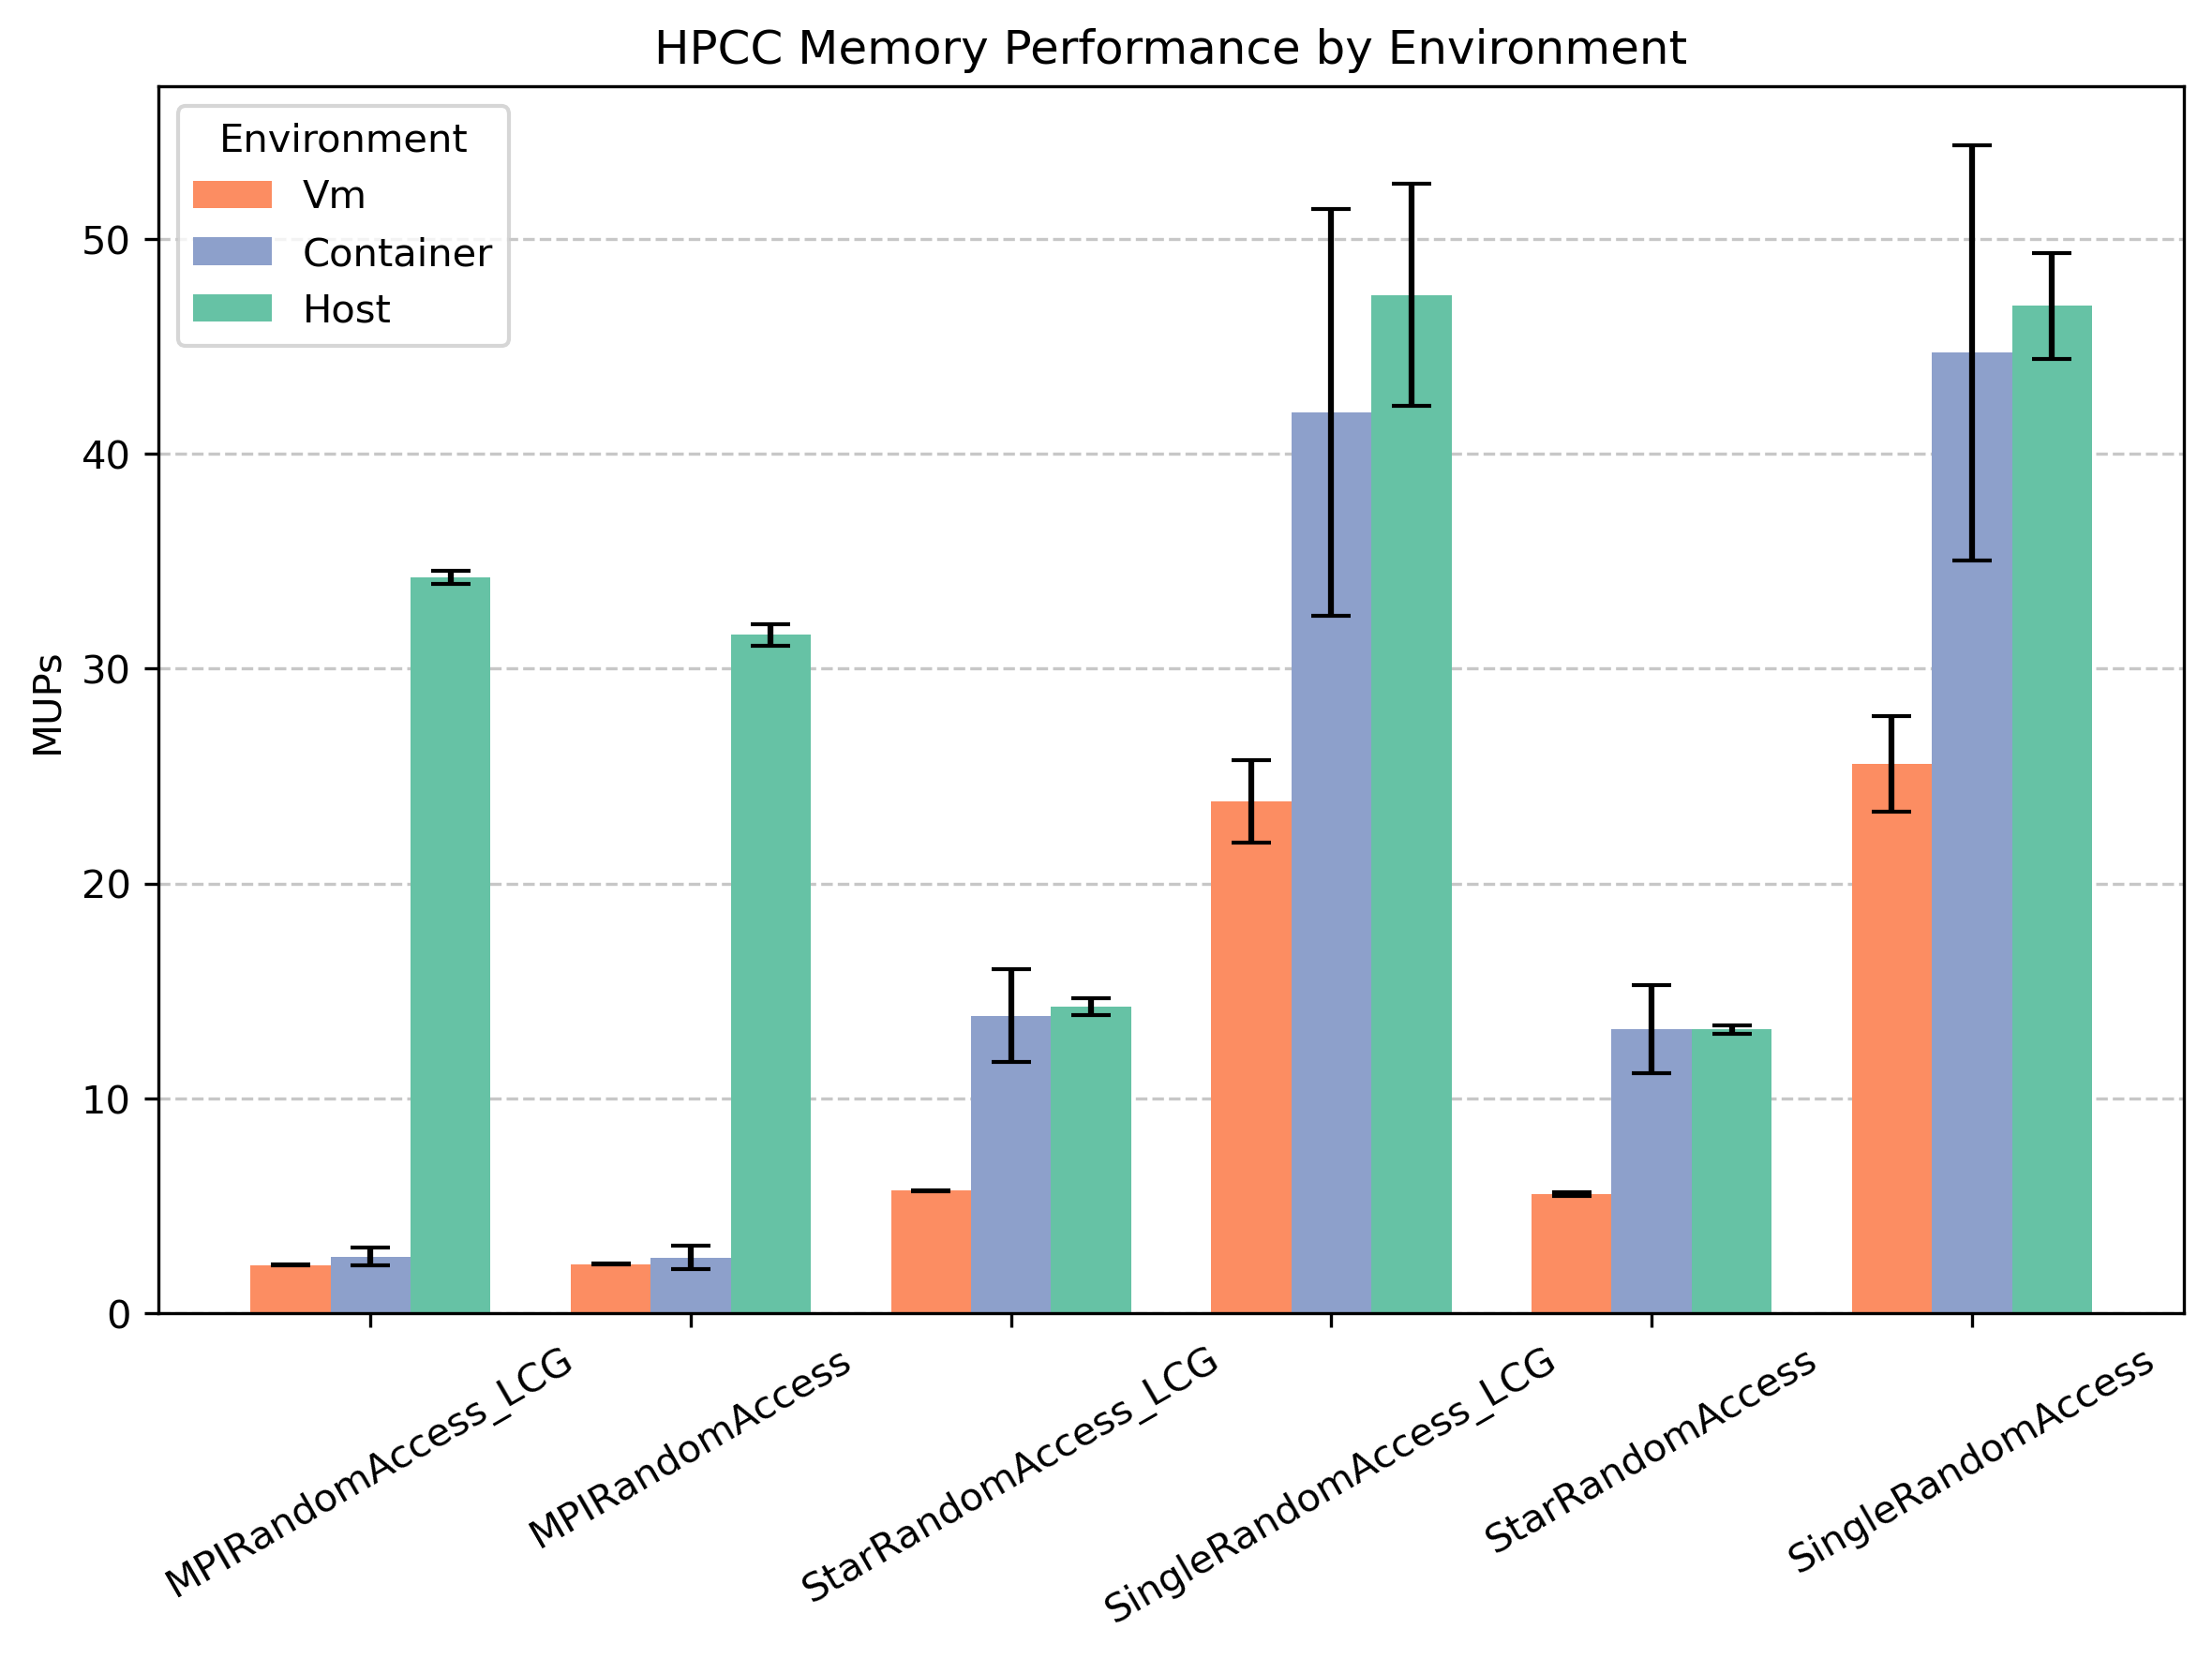
\includegraphics[width=0.8\linewidth]{assets/hpcc_memory_performance.png}
    \caption{Memory Random Access Benchmarks: VM (orange) vs Container (blue) vs Host (green). All the benchmarks are reported in mega updates per second (MUP/s).}
    \label{fig:hpcc_memory_performance}
\end{figure}

\subsubsection{Latency and Bandwidth}

The ping-pong benchmark is a fundamental test used to measure the performance of a communication channel or link between two endpoints. In a cluster environment, a ping-pong benchmark is typically run between two different nodes. On a single host machine, a ping-pong benchmark is typically run between two processes or threads running on that same machine. For this reason here the Host results are not a proper baseline to compare the VMs and container results.

From the table \ref{tab:pingpong} we can see that VM introduces massive latency penalties with respect to the Containers. Analogously, for the bandwidth the containers show the best performances. 

\begin{table}[htbp]
\centering
\renewcommand{\arraystretch}{1.2}
\begin{tabular}{lccc}
\toprule
\textbf{Benchmark} & \textbf{VM} & \textbf{Container} & \textbf{Host} \\
\midrule
\multicolumn{4}{l}{\textbf{Latency (µs)}} \\
MinPingPong             & 1.957 ± 0.066 & 1.853 ± 0.056 & 0.201 ± 0.004 \\
AvgPingPong              & 49.026 ± 1.597 & 6.855 ± 0.600 & 0.211 ± 0.005 \\
MaxPingPong              & 75.651 ± 2.980 & 9.962 ± 1.540 & 0.218 ± 0.004 \\
NaturallyOrderedRing    & 61.426 ± 7.146 & 5.926 ± 0.376 & 0.227 ± 0.005 \\
RandomlyOrderedRing     & 63.771 ± 8.449 & 6.872 ± 0.332 & 0.230 ± 0.003 \\
\midrule
\multicolumn{4}{l}{\textbf{Bandwidth (GB/s)}} \\
MinPingPong            & 0.230 ± 0.025 & 4.995 ± 1.033 & 11.517 ± 0.725 \\
AvgPingPong            & 3.617 ± 0.422 & 7.943 ± 0.674 & 12.750 ± 0.212 \\
MaxPingPong            & 11.383 ± 1.381 & 13.726 ± 0.278 & 13.908 ± 0.468 \\
NaturallyOrderedRing  & 0.145 ± 0.020 & 2.064 ± 0.115 & 3.101 ± 0.021 \\
RandomlyOrderedRing   & 0.120 ± 0.014 & 1.857 ± 0.020 & 2.971 ± 0.073 \\
\bottomrule
\end{tabular}
\caption{Latency and Bandwidth Benchmark: VM vs Container vs Host. The values are reported as mean ± standard deviation, calculated over three measurements ($n = 3$).}
\label{tab:pingpong}
\end{table}

\begin{figure}[htbp]
    \centering
    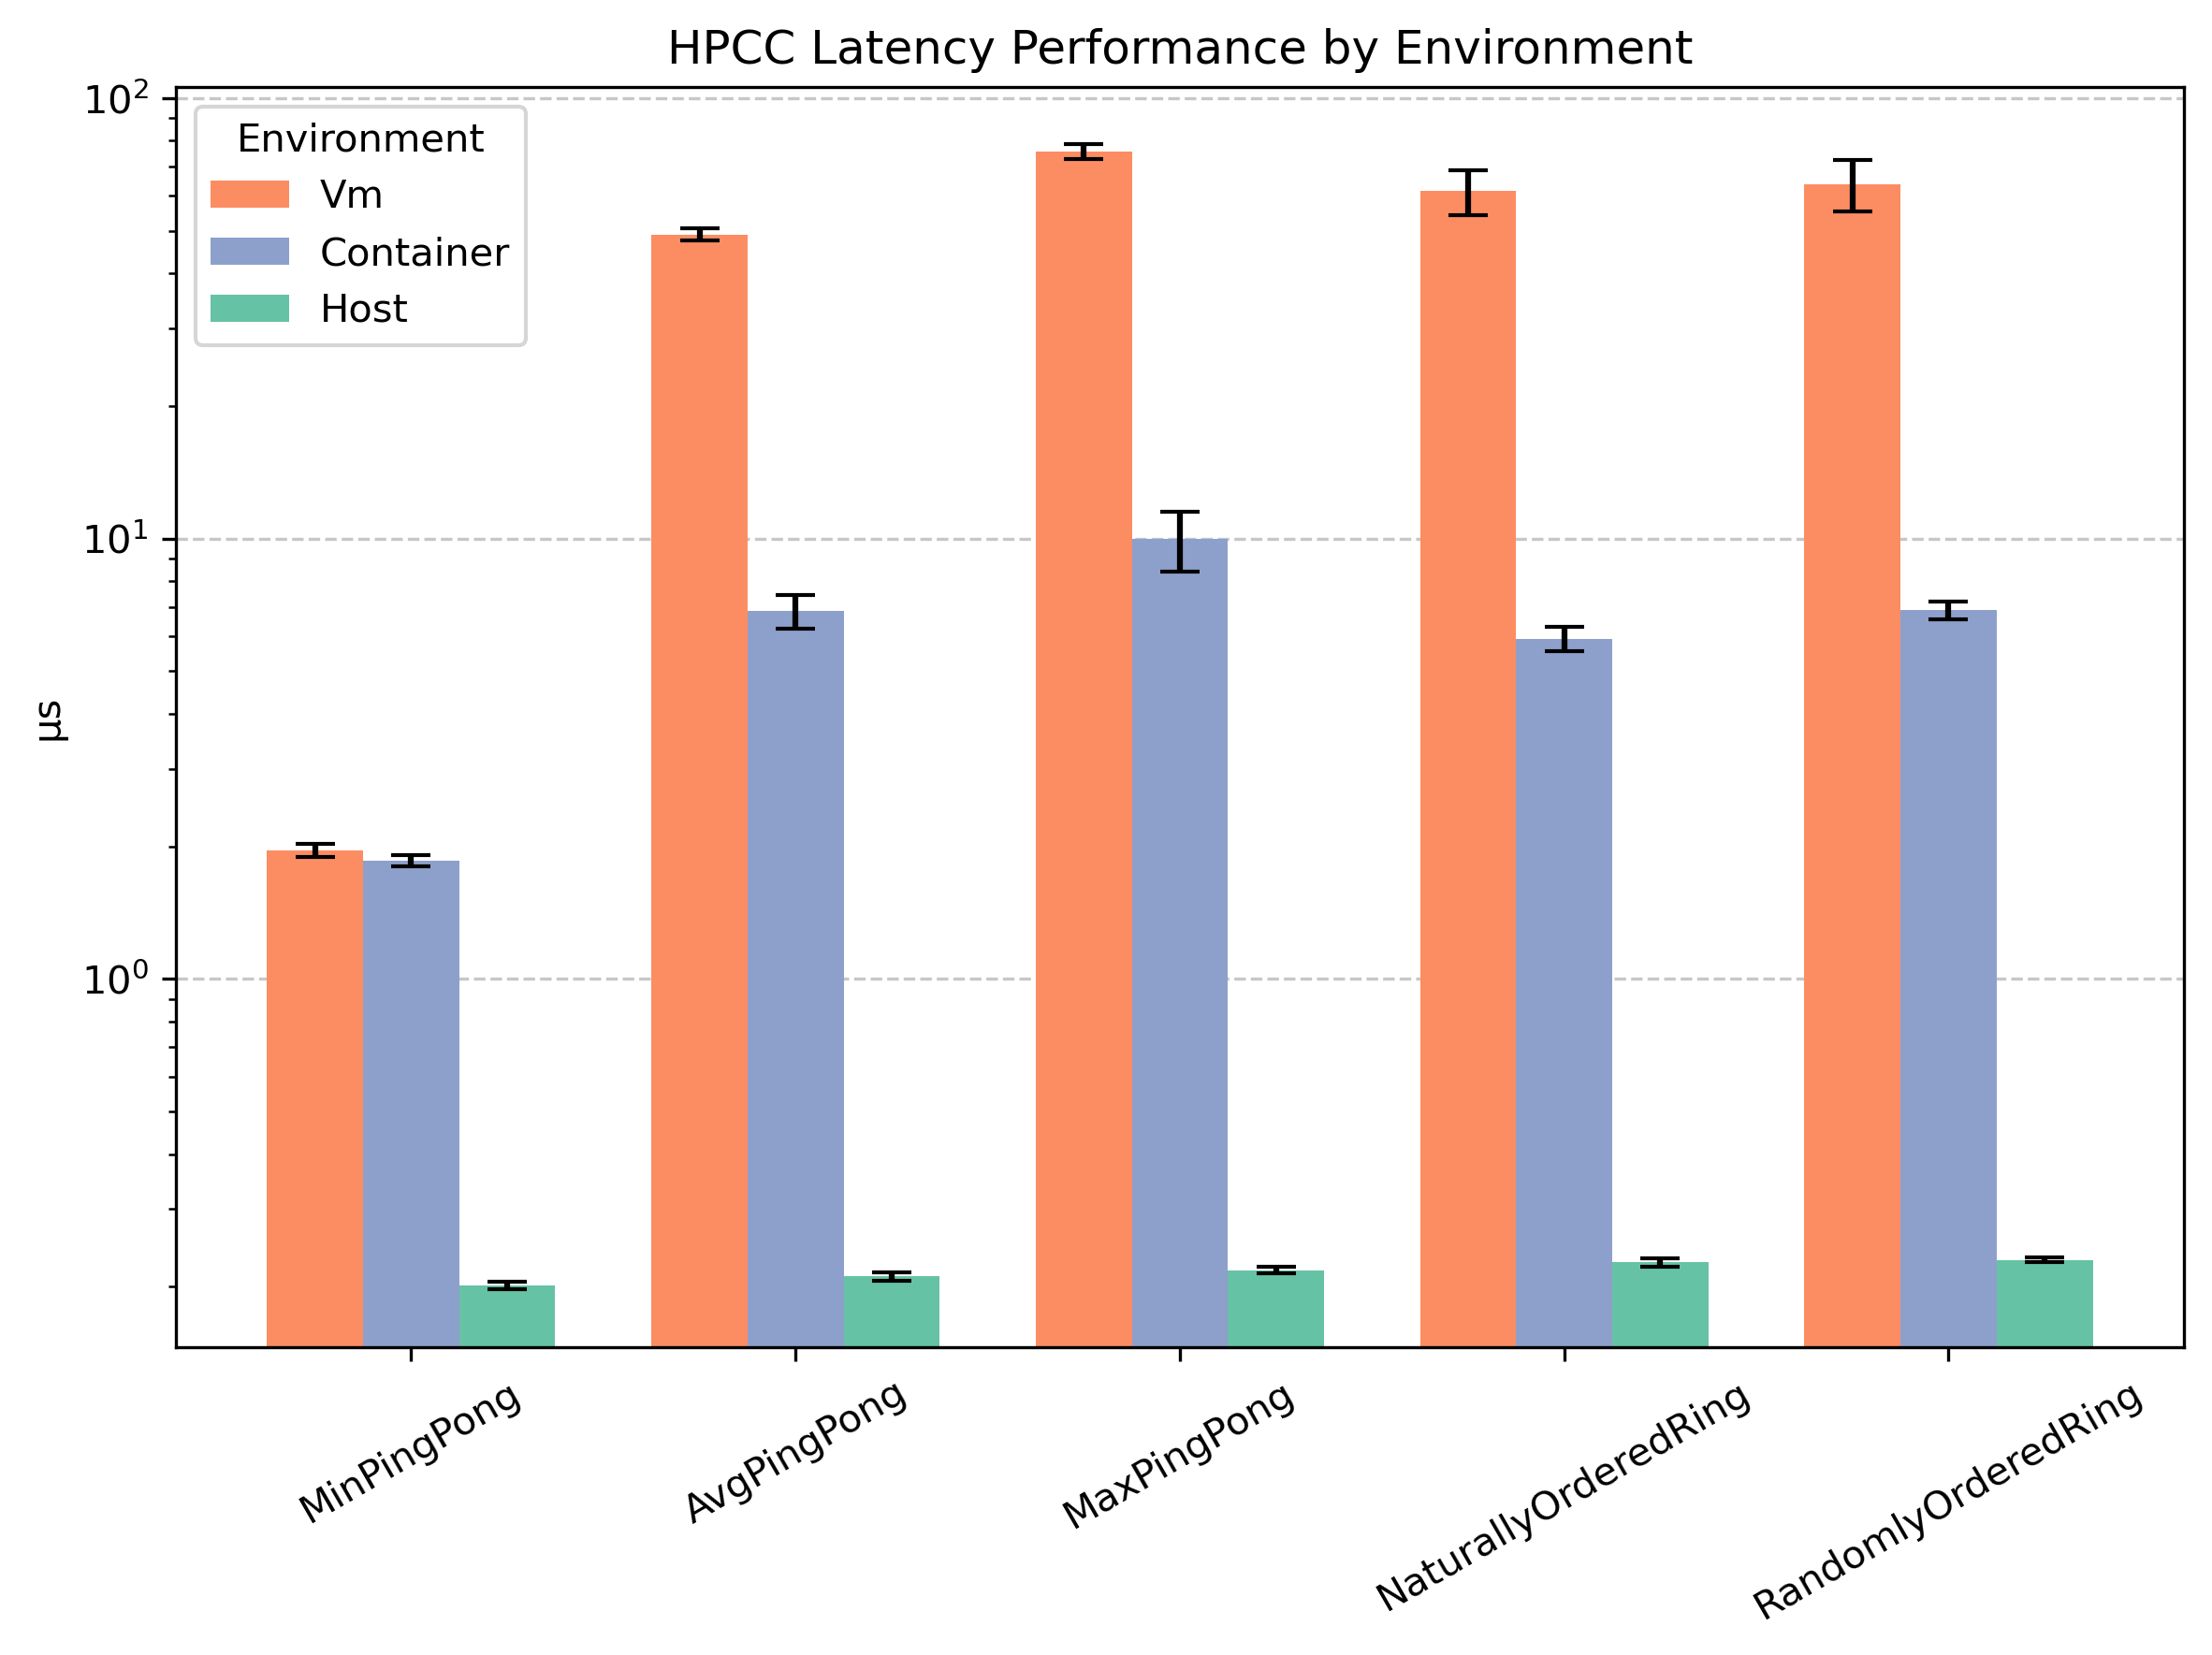
\includegraphics[width=0.8\linewidth]{assets/hpcc_latency_performance.png}
    \caption{Latency and Bandwidth Benchmarks: VM (orange) vs Container (blue) vs Host (green). All the latencies are reported in microseconds (µs) and y-axis is in log scale.}
    \label{fig:hpcc_latency_performance}
\end{figure}

\subsection{stress-ng}

According to the stress-ng documentation\footnote{\url{https://wiki.ubuntu.com/Kernel/Reference/stress-ng}}, the tool reports a stress test's ``throughput" in terms of bogus operations per second (bogo-ops). As highlited in the documentation, it is important to point out that the size and nature of a bogo-op vary depending on the specific stressor being used, making throughput values incomparable across different stressors.

For the CPU stressor, both the host and the container environments demonstrate nearly identical performance. The minor variability observed between them falls well within the expected margin of experimental variation. In contrast, the VM environment exhibits significantly lower throughput -- approximately 31\% lower than that of the host and container. This degradation in performance is likely attributable to the overhead introduced by the virtualization layer of the hypervisor. A similar trend is observed in the memory stressor results. The VM configuration again yields the lowest performance, falling significantly behind both the host and the container environments, which perform comparably to one another.

For this test, two time metrics are of particular interest: Real Time (or wall-clock time), which measures the total elapsed time for the benchmark from start to finish, and Usr+Sys Time (CPU time), which represents the cumulative time the process spent executing in user and system modes. We observe that in general for the CPU stressor, the Real Time and Usr+Sys Time metrics are nearly identical for each environment. This means that the cores are fully utilized during the benchmark, and there is no significant overhead from context switching or other system activities. The system has enough cores (e.g., 4 physical cores for 4 threads) and each thread gets its own core and runs simultaneously. For the memory stressor instead, the Real Time and Usr+Sys Time metrics diverge significantly in the host and container environments. Containers run directly on the host kernel with near-native performance, the divergence in the two times could come from the fact that containers can use memory more efficiently and in full parallel, so each thread contributes more actual CPU time. In this way Usr+Sys time becomes higher than wall-clock time due to summed per-thread CPU time. This asymmetry is notably less pronunced in the VM environment. One possible explanation is that VMs don't access physical memory directly — they go through a virtual memory layer managed by the hypervisor. The net result is that threads are slower, not all the cores are used and less cumulative CPU time is used.
The test has been repeated five times for each stressor.

\begin{table}[htbp]
    \centering
    \begin{tabular}{lccc}
    \toprule
    \textbf{Benchmark} & \textbf{VM} & \textbf{Container} & \textbf{Host} \\
    \midrule
    \textbf{CPU (kBOps/s)} & & & \\
    Real Time & $0.924 \pm 0.008$ & $1.340 \pm 0.013$ & $1.348 \pm 0.016$ \\
    Usr+Sys Time & $0.926 \pm 0.008$ & $1.342 \pm 0.013$ & $1.349 \pm 0.016$ \\
    \midrule
    \textbf{Memory (kBOps/s)} & & & \\
    Real Time & $40.183 \pm 0.265$ & $52.180 \pm 5.025$ & $53.900 \pm 4.948$ \\
    Usr+Sys Time & $41.434 \pm 0.952$ & $66.543 \pm 2.954$ & $62.687 \pm 3.254$ \\
    \bottomrule
    \end{tabular}
    \caption{Stress-ng results for VM, Container, and Host environments. The values are reported as mean ± standard deviation, calculated over five measurements ($n = 5$).}
    \label{tab:stress-ng}
\end{table}


\subsection{sysbench}

Sysbench provides several test. The key metrics for the CPU benchmarking are Evets/s that measures how many test events the system can handle per second, so the higher the better. And the latency sum that measures the total latency for all executed events, which gives a measure of how long it took to complete all tasks. For the memory benchmark the key metric is the transfer rate, \textit{i.e.}, the memory bandwidth expressed in Gib/s.

The CPU performance are largely consistent across all three environments, with containers achieving slightly better results. For the memory instead we have a clear winner. The container cluster consistently delivers the highest memory bandwidth, outperforming both the VM cluster and the single-host configuration. The VM cluster, in particular, demonstrates a substantial bottleneck in memory performance, indicating inefficiencies in its virtualized memory subsystem. While the single host achieves respectable memory throughput, it does not match the peak performance seen in the container environment. Cumulative latency figures reinforce the efficiency of the container-based setup and highlight the significant memory handling limitations present in the VM cluster.
The test has been repeated five times for both CPU and memory. 

\begin{table}[htbp]
    \centering
    \begin{tabular}{lccc}
    \toprule
    \textbf{Benchmark} & \textbf{VM} & \textbf{Container} & \textbf{Host} \\
    \midrule
    \textbf{CPU} & & & \\
    Events/s & $453.97 \pm 1.28$ & $459.74 \pm 2.54$ & $452.38 \pm 6.76$ \\
    Latency sum (ms) & $9998.15 \pm 0.70$ & $9999.55 \pm 0.51$ & $9999.56 \pm 0.72$ \\
    \midrule
    \textbf{Memory} & & & \\
    Bandwidth (Gib/s) & $3.88 \pm 0.02$ & $5.51 \pm 0.09$ & $5.19 \pm 0.08$ \\
    Latency sum (ms) & $1066.09 \pm 8.01$ & $839.99 \pm 14.63$ & $895.79 \pm 18.40$ \\
    \bottomrule

    \end{tabular}
    \caption{Sysbench performance metrics for VM, Container, and Host environments. The values are reported as mean ± standard deviation, calculated over five measurements ($n = 5$).}
    \label{tab:sysbench}
\end{table}


\subsection{IOZone}

The Iozone benchmark tests file I/O performance for the following operations: read, write, re-read, re-write, read backwards, read strided, fread, fwrite, random read/write, pread/pwrite variants. Here are reported the the results for the main operations both for vm and containers: read, write, random read, random write. In the following plots (figure \ref{fig:reader local and shared}, \ref{fig:writer local and shared}, \ref{fig:random read local and shared}, \ref{fig:random write local and shared}) we have on the x-axis the file size (KB), on the y-axis the block size (KB) and on the z one the throughput (MB/s).
The File size is the size of the file being tested. The transfer size (or Block size) is the size of the I/O operations performed during the test.
The Throughput represents how fast data was read during the benchmark using a particular combination of file size and transfer size.

Let's consider for example the results for the \textbf{reader} test, Figure \ref{fig:reader local and shared}. Immediately we can note, from the changing in the reference throughput scale (z axis) that there is a significant difference when going from the local file system to the shared one. Moreover, when going from the local to the shared system it is evident that container cluster outperform the VM one. This consideration is in general true also for all the other tests reported below in figure \ref{fig:writer local and shared}, \ref{fig:random read local and shared}, \ref{fig:random write local and shared}.

\begin{figure}[H]
    \centering
    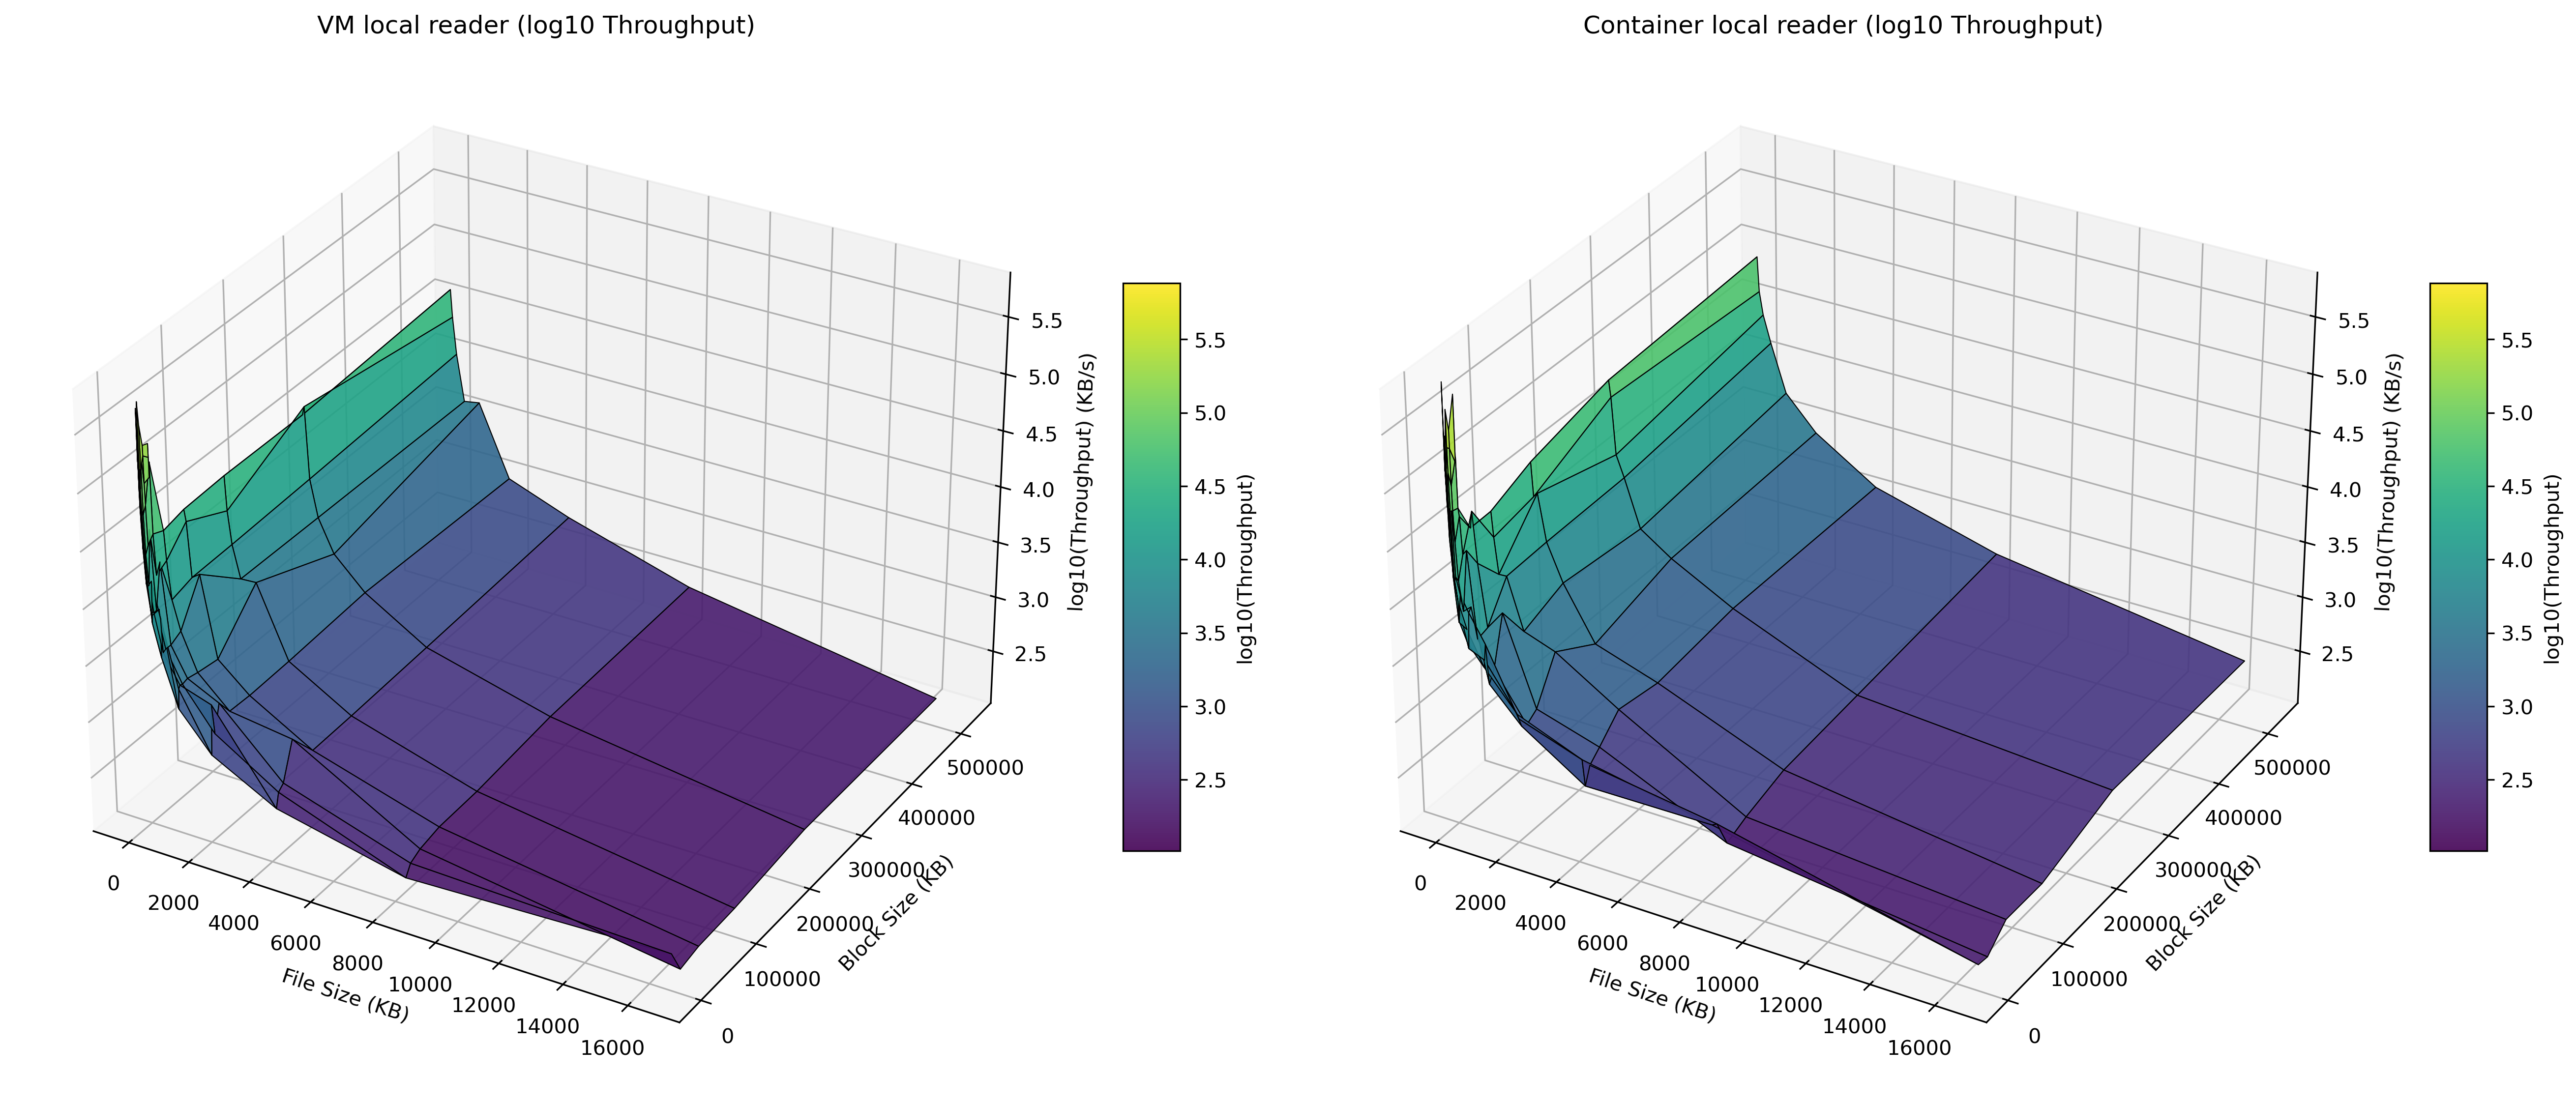
\includegraphics[width=\linewidth]{assets/VM local reader_Container local reader_log_surfaces.png}
    \end{figure}
\begin{figure}[H]
    \centering
    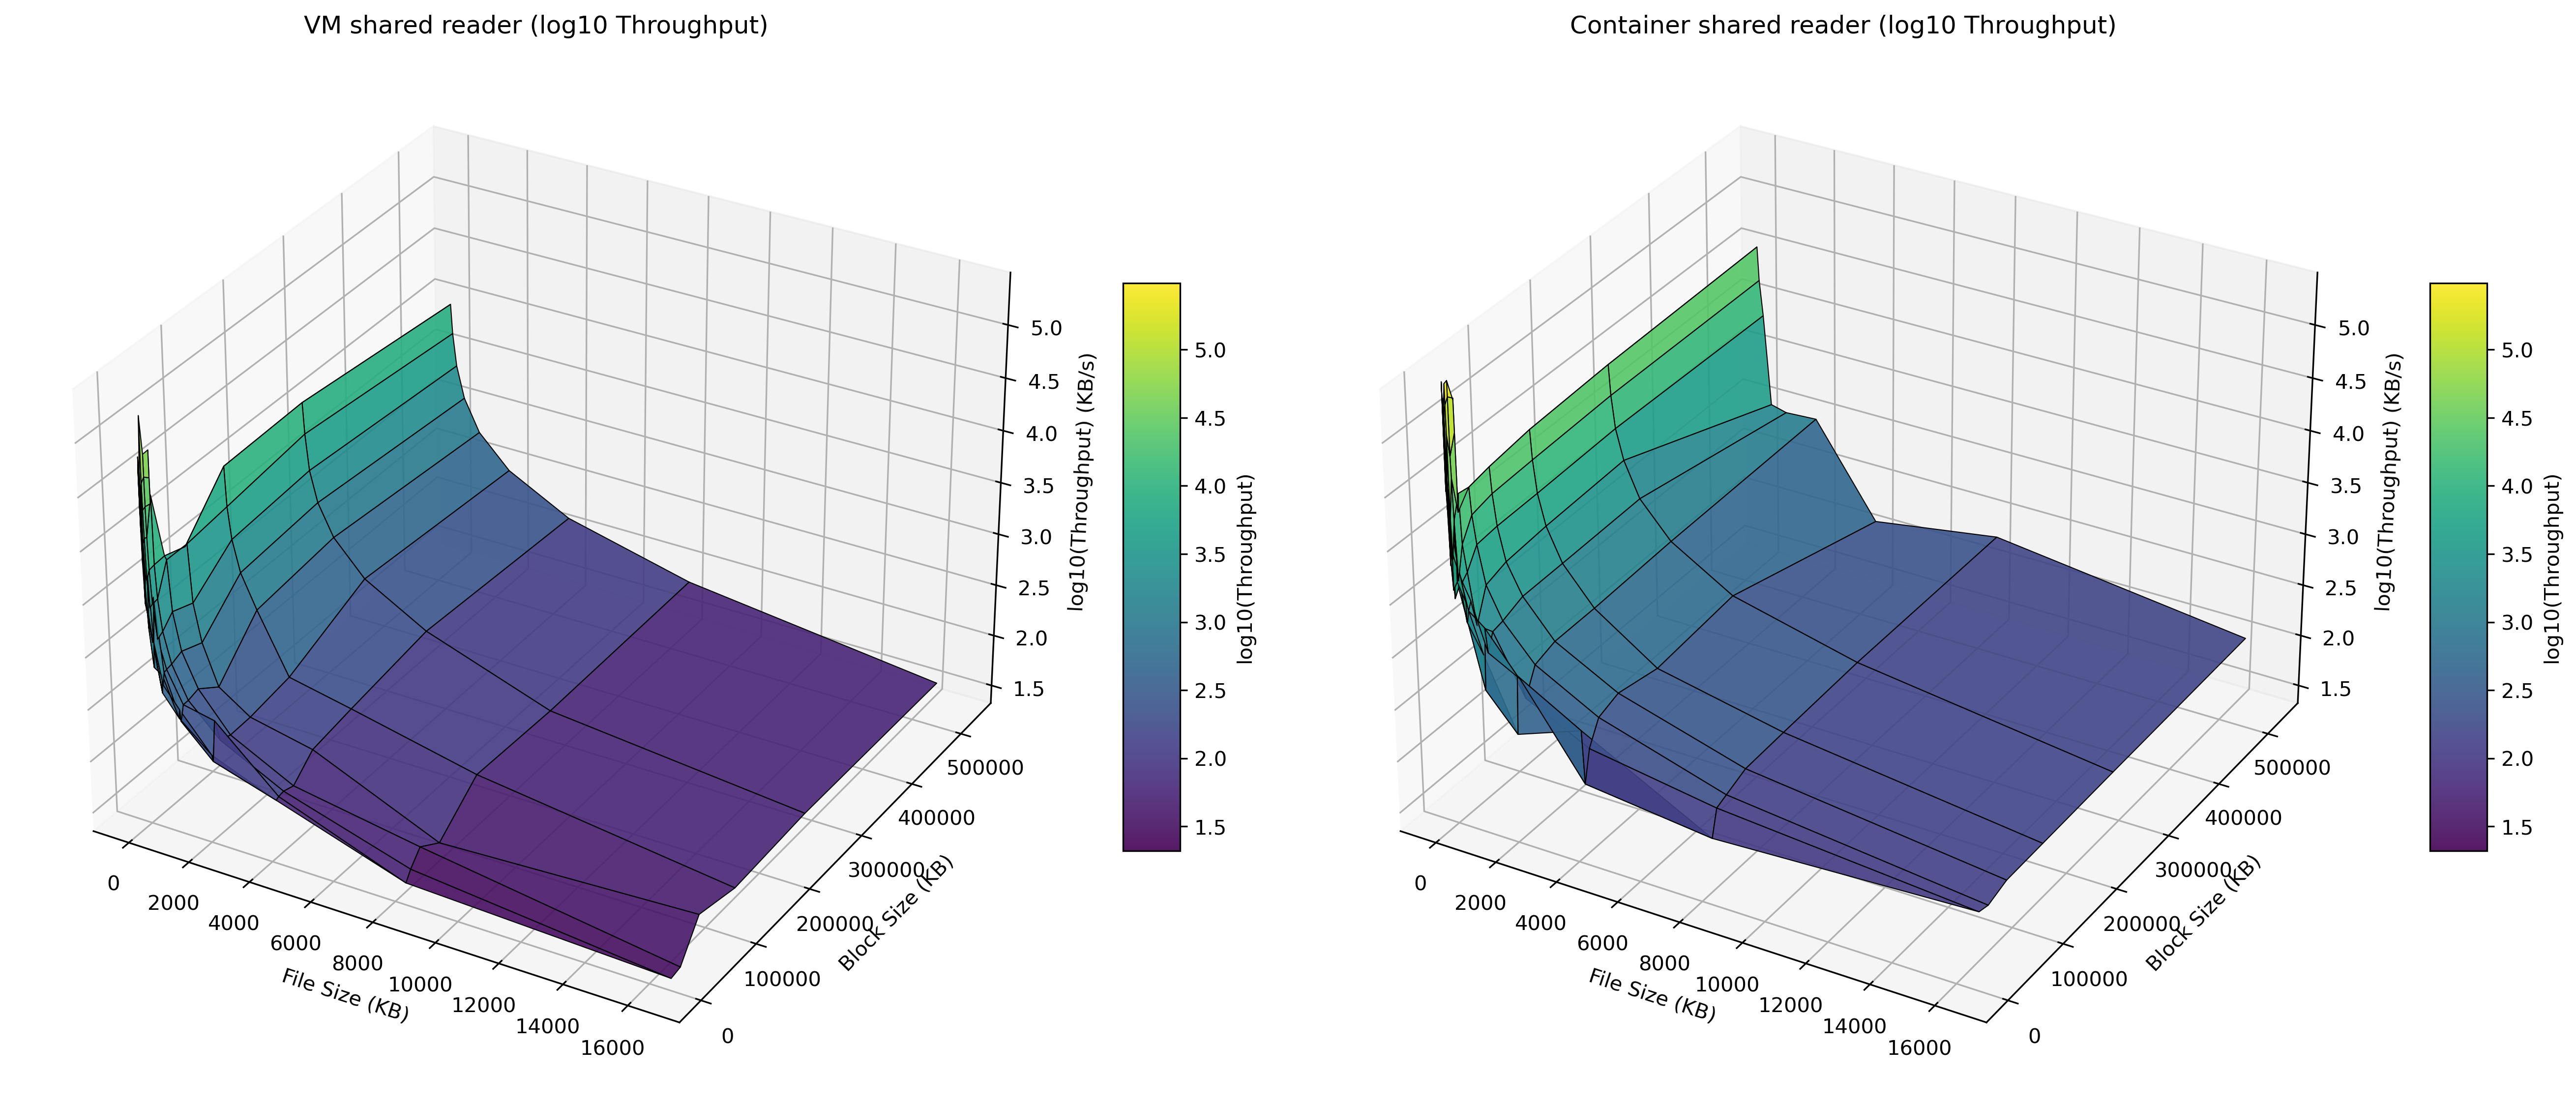
\includegraphics[width=\linewidth]{assets/VM shared reader_Container shared reader_log_surfaces.png}
    \caption{local and shared reader report}
    \label{fig:reader local and shared}
\end{figure}

\begin{figure}[H]
    \centering
    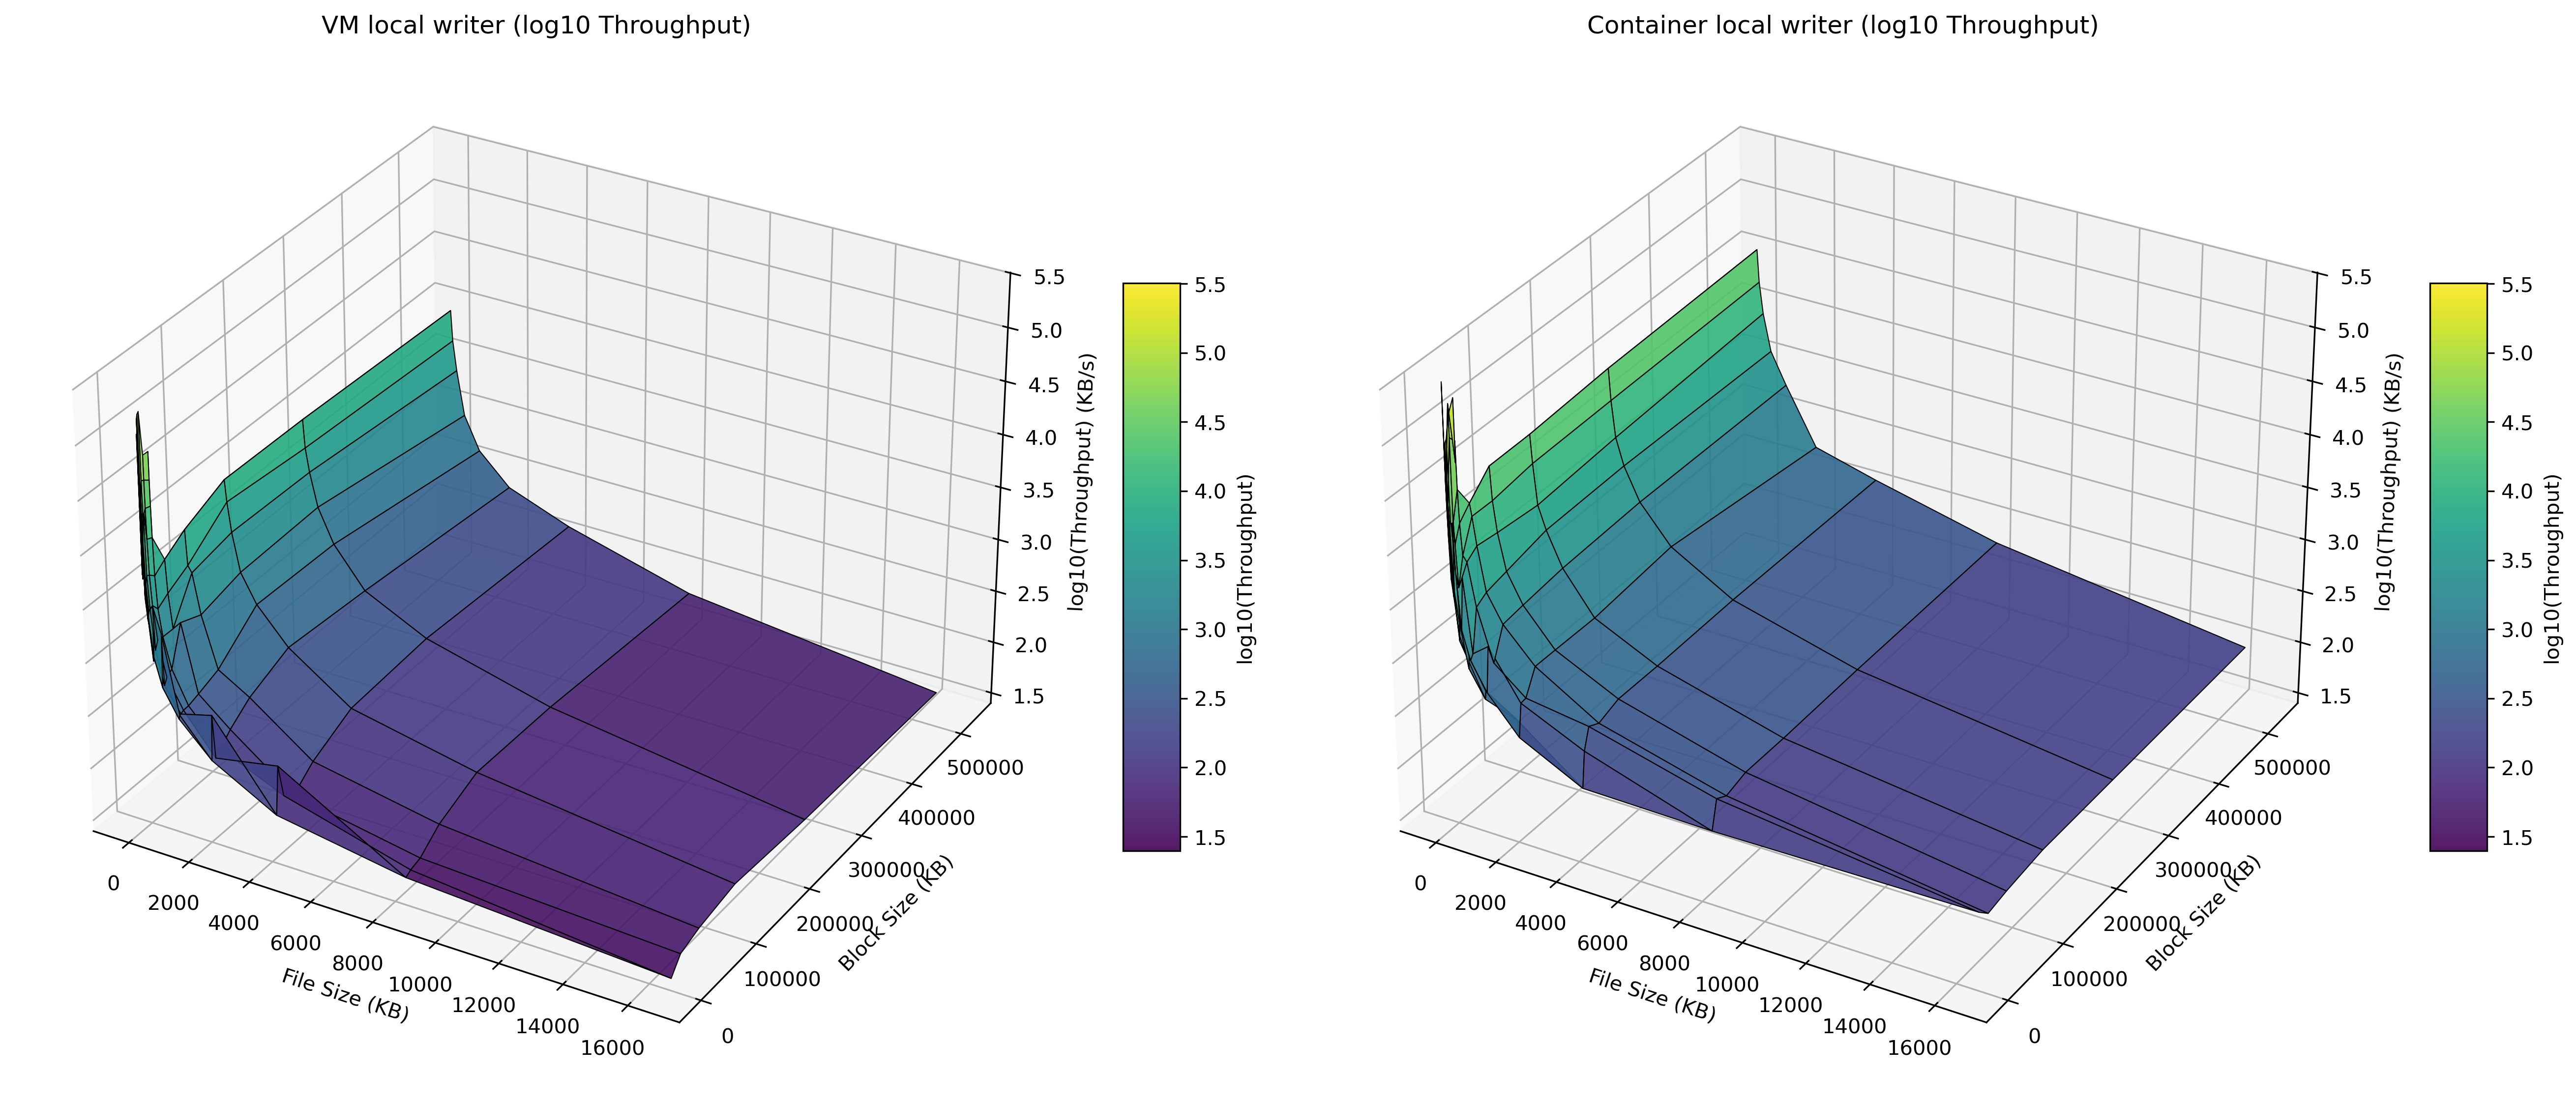
\includegraphics[width=\linewidth]{assets/VM local writer_Container local writer_log_surfaces.png}
        \end{figure}
\begin{figure}[H]
    \centering
    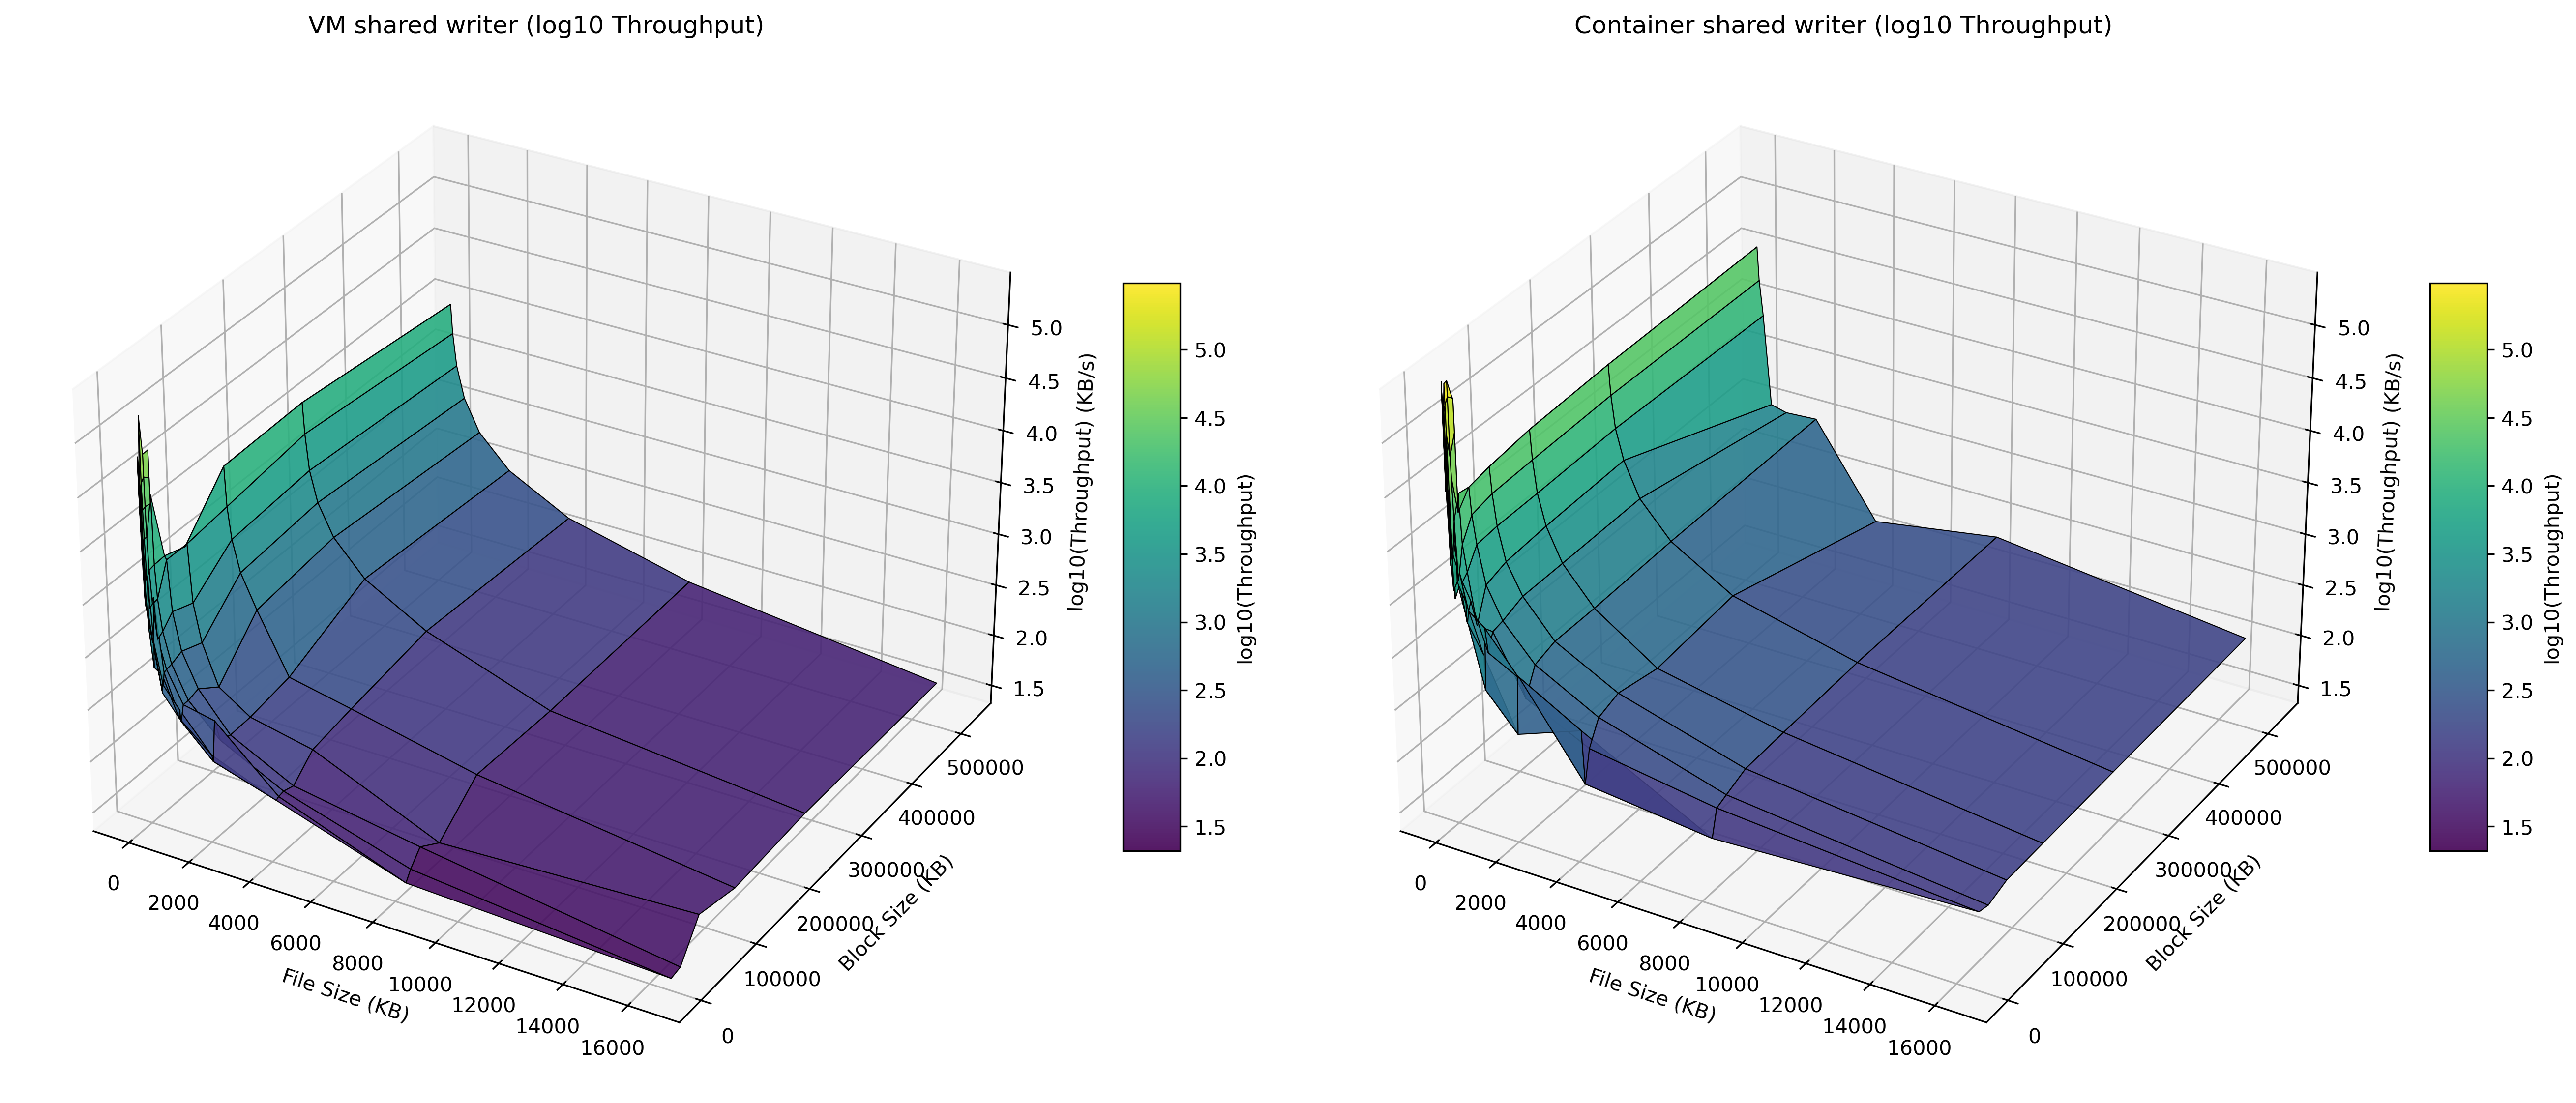
\includegraphics[width=\linewidth]{assets/VM shared writer_Container shared writer_log_surfaces.png}
    \caption{local and shared writer report}
    \label{fig:writer local and shared}
\end{figure}

\begin{figure}[H]
    \centering
    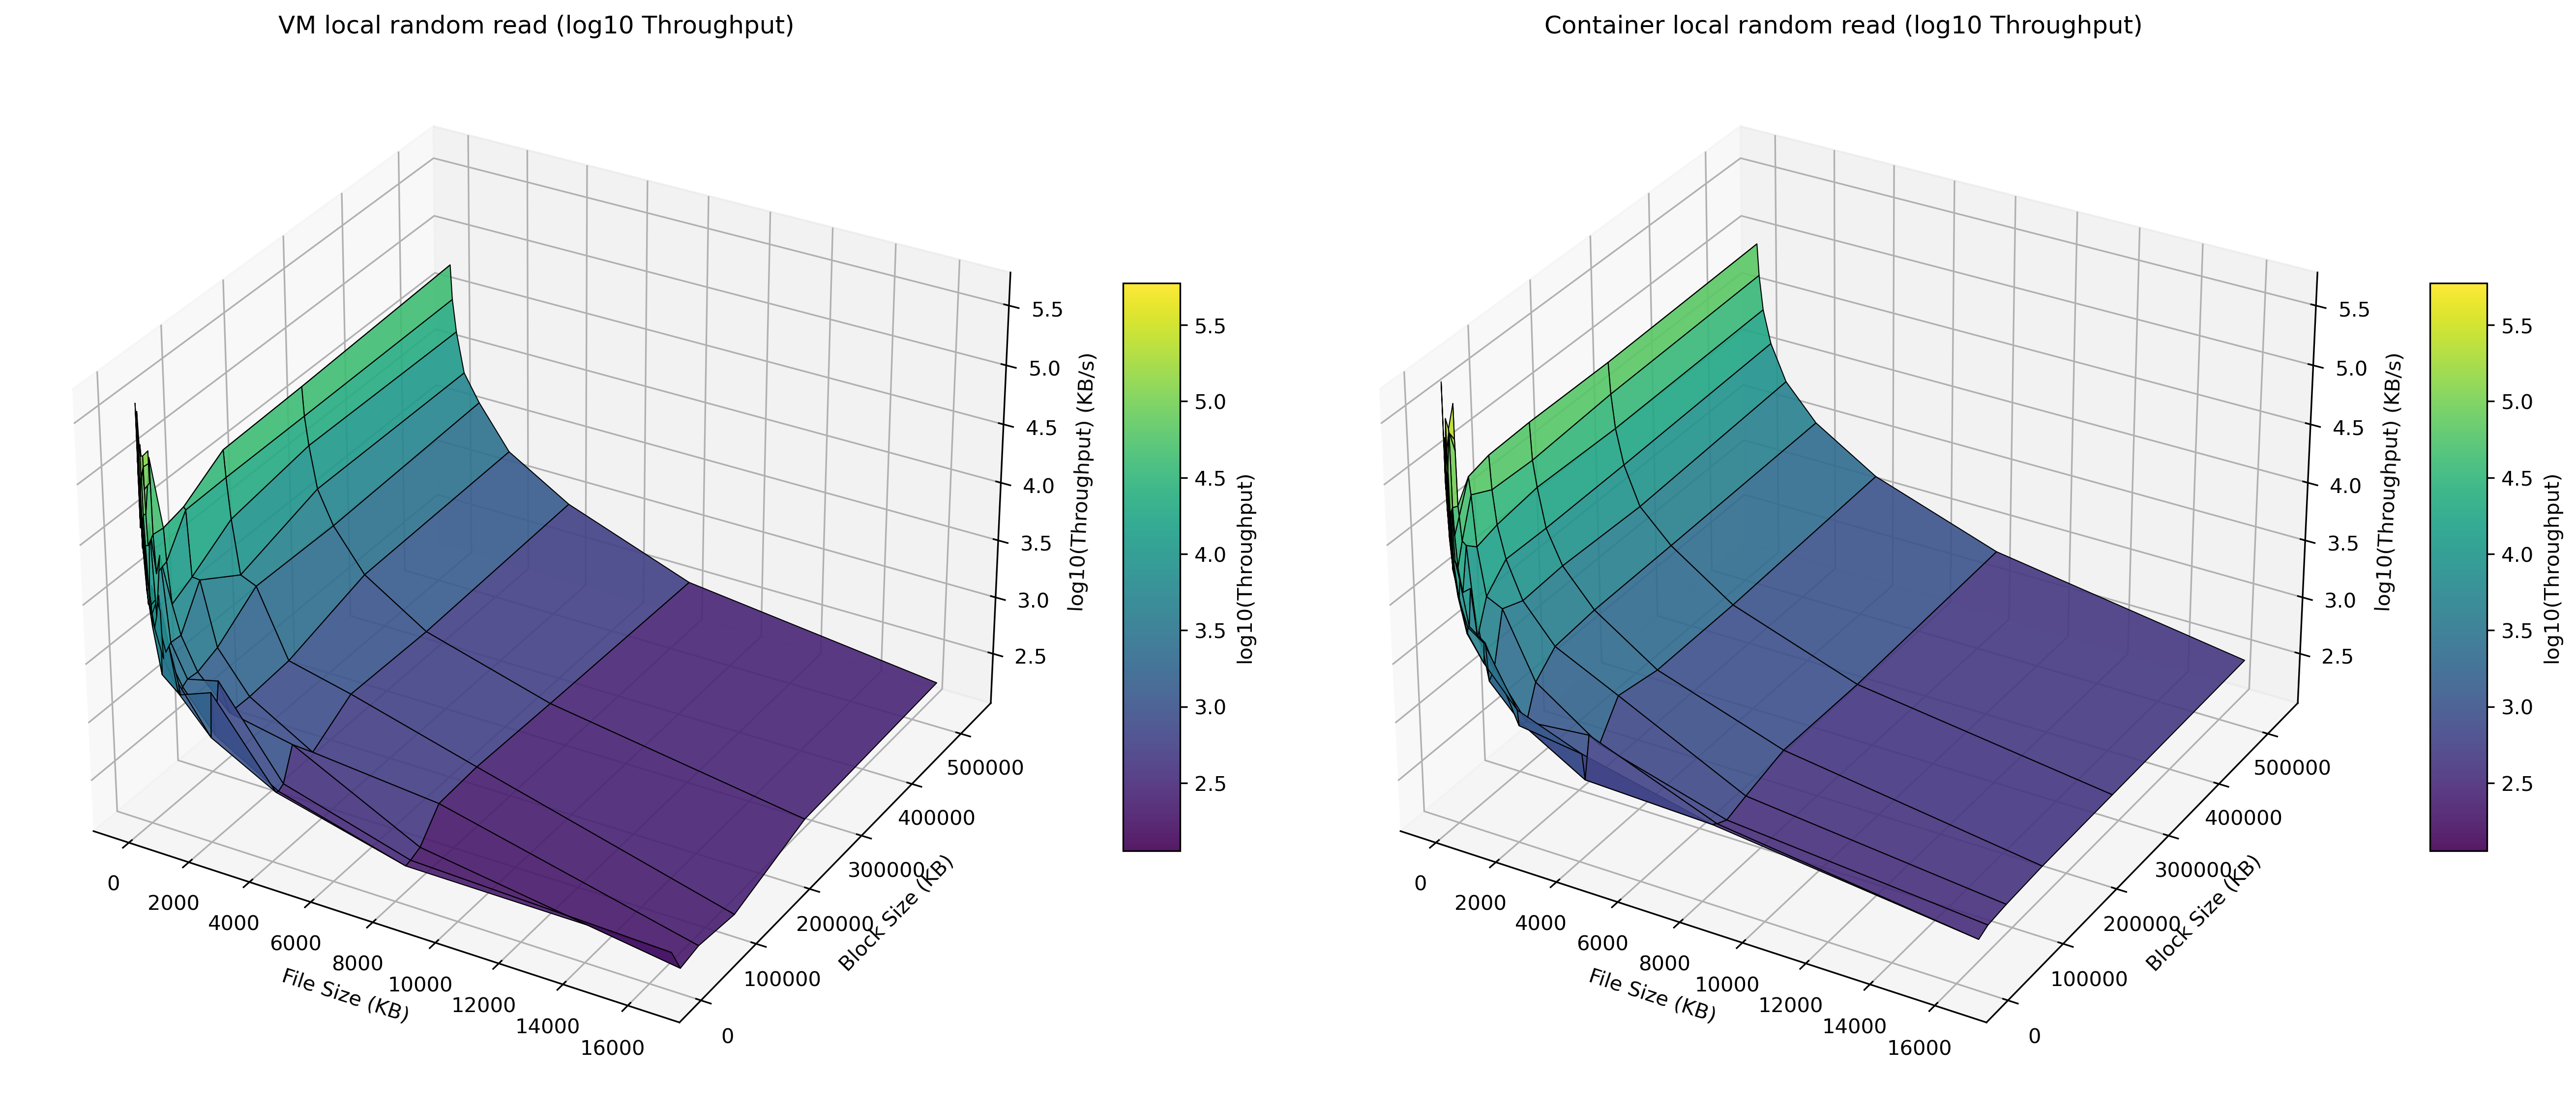
\includegraphics[width=\linewidth]{assets/VM local random read_Container local random read_log_surfaces.png}
        \end{figure}
\begin{figure}[H]
    \centering
    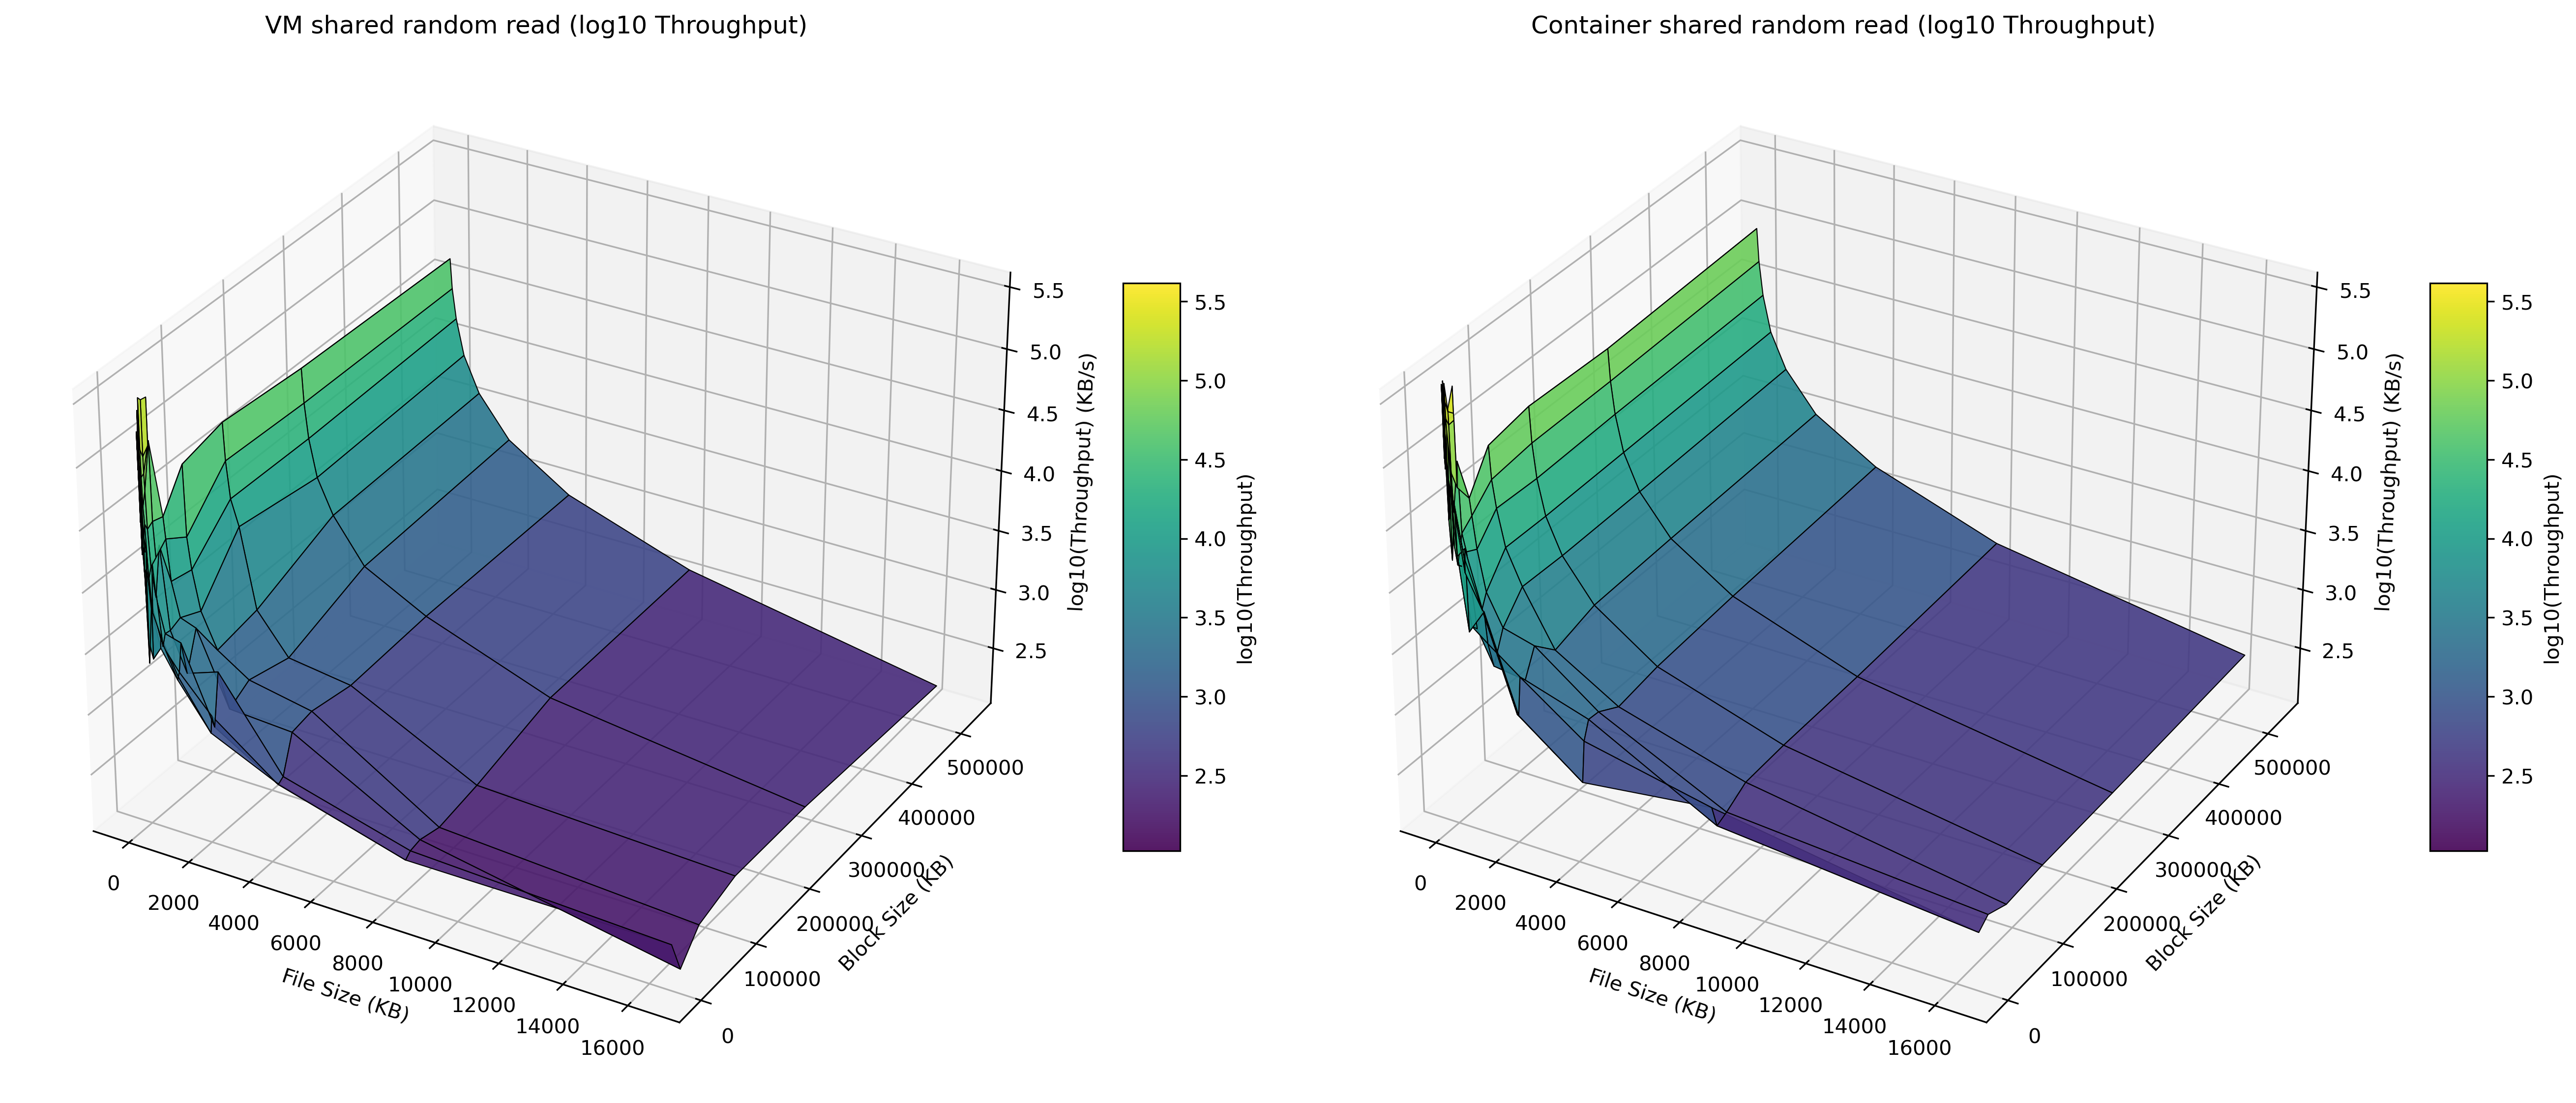
\includegraphics[width=\linewidth]{assets/VM shared random read_Container shared random read_log_surfaces.png}
    \caption{local and shared random read report}
    \label{fig:random read local and shared}
\end{figure}

\begin{figure}[H]
    \centering
    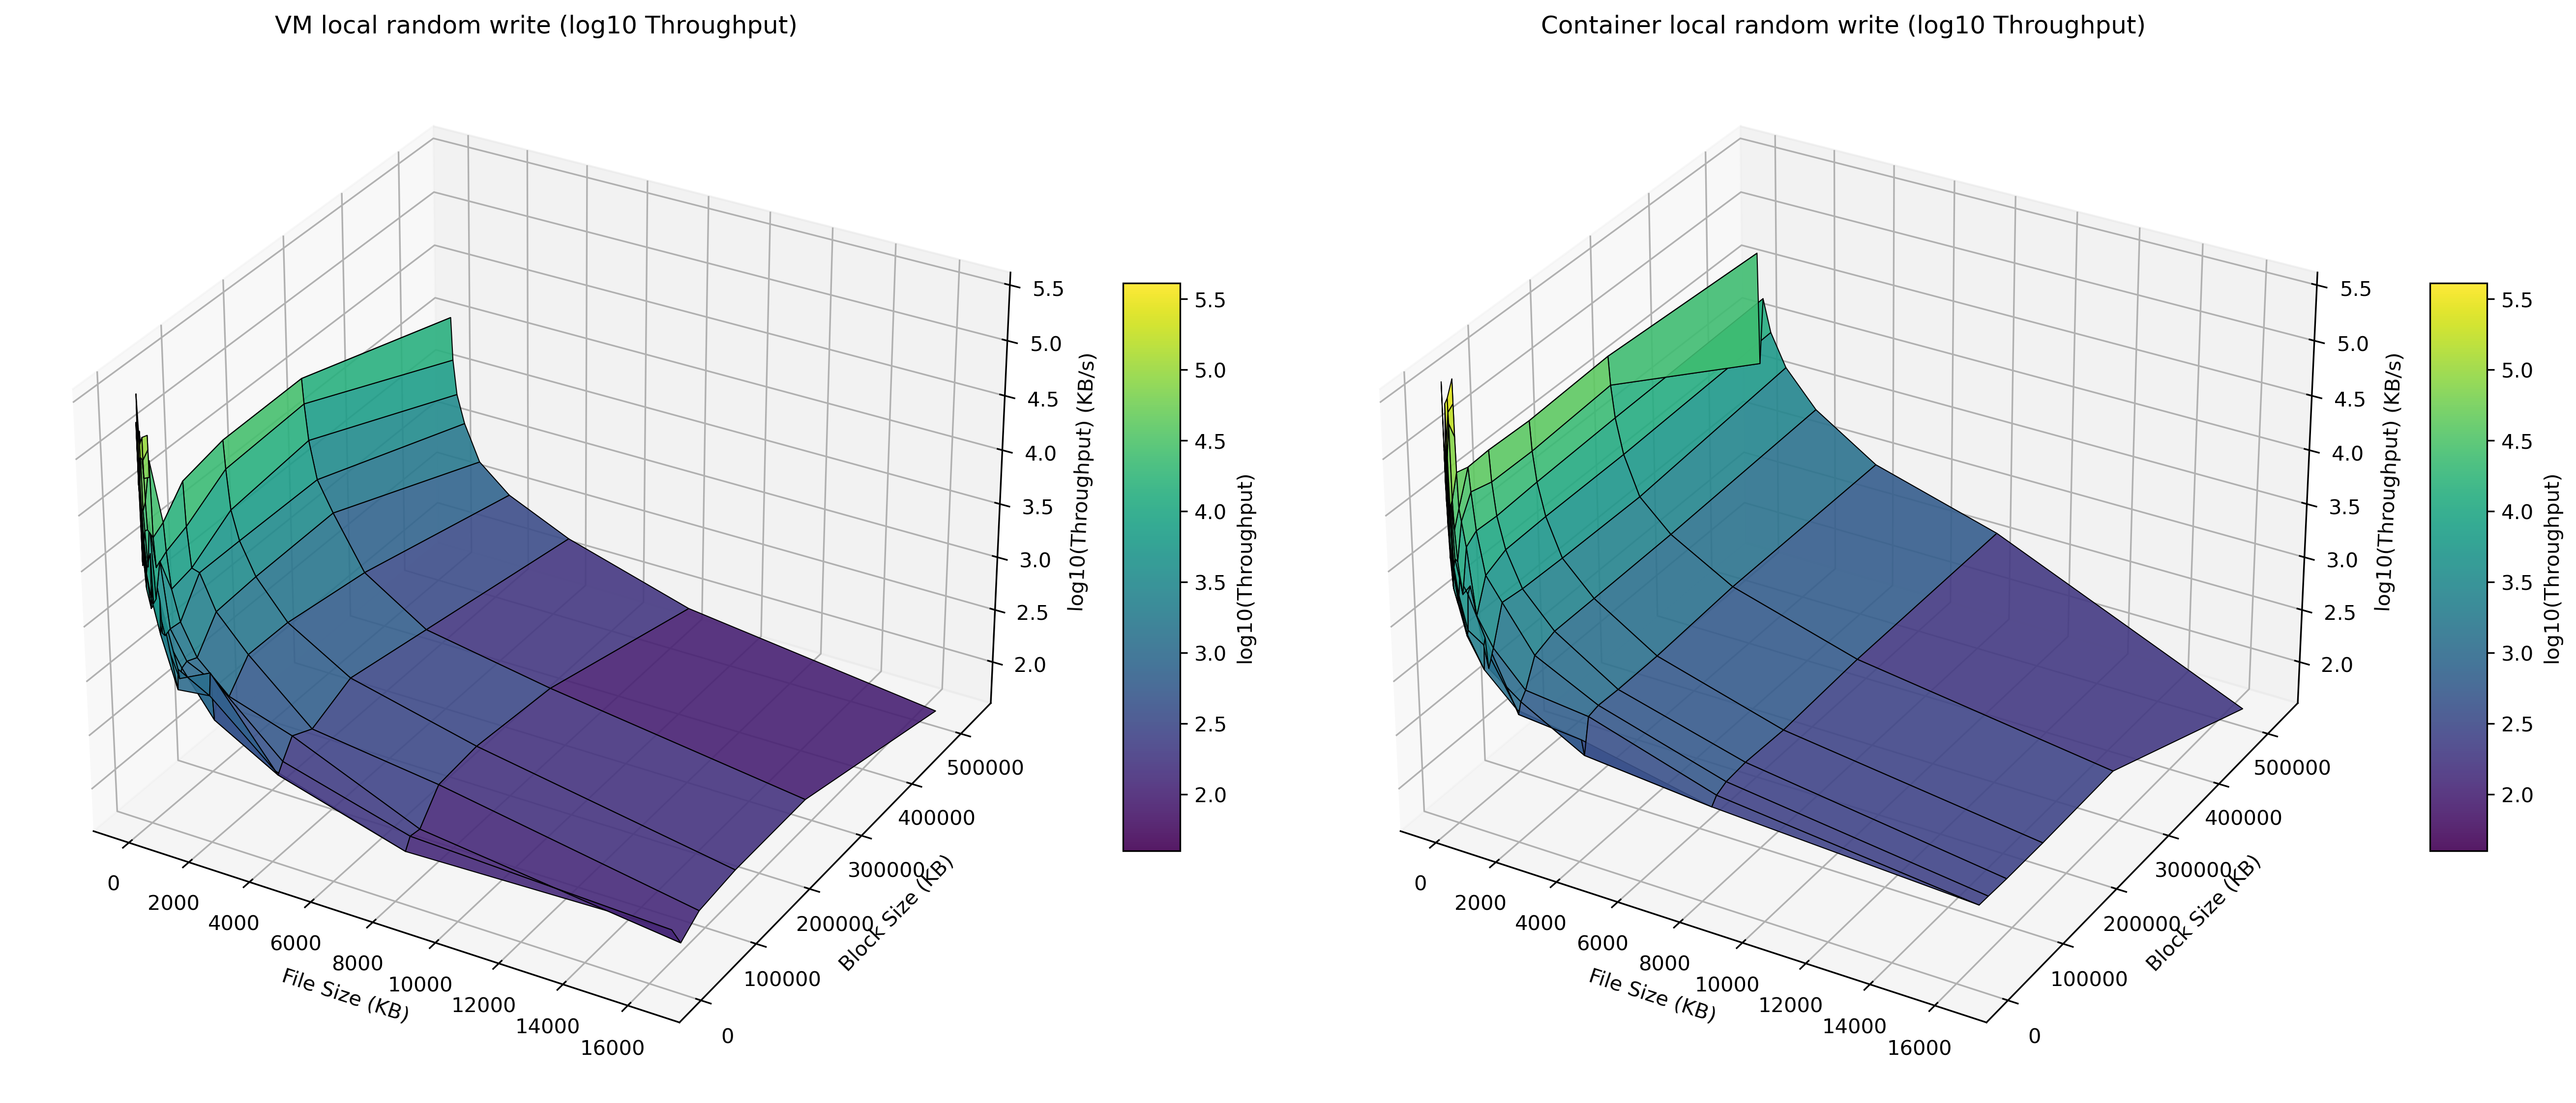
\includegraphics[width=\linewidth]{assets/VM local random write_Container local random write_log_surfaces.png}
        \end{figure}
\begin{figure}[H]
    \centering
    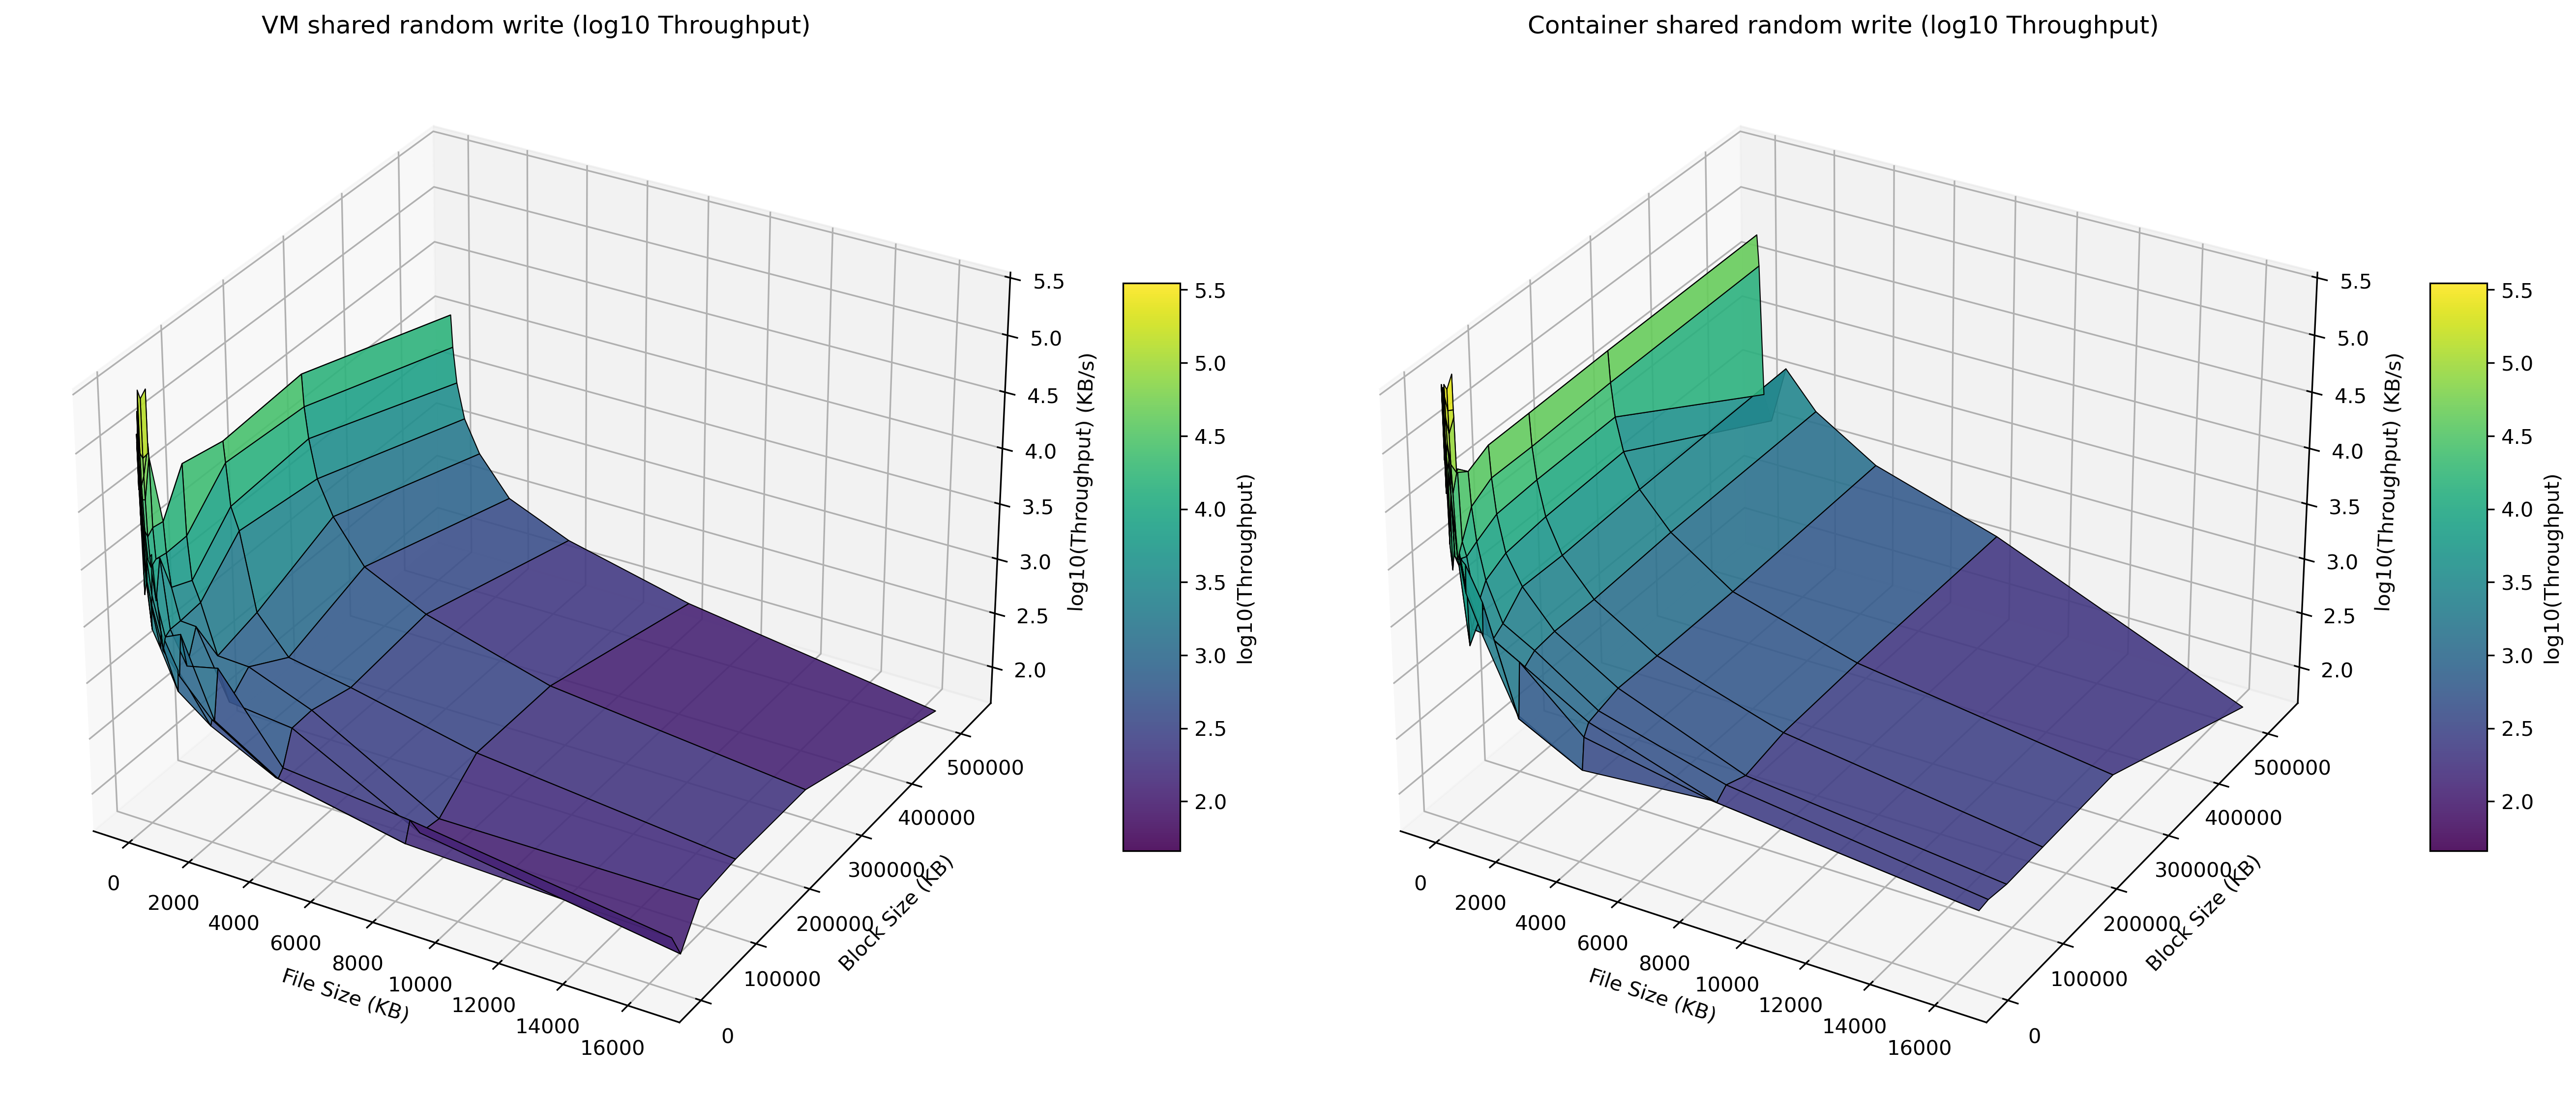
\includegraphics[width=\linewidth]{assets/VM shared random write_Container shared random write_log_surfaces.png}
    \caption{local and shared random write report}
    \label{fig:random write local and shared}
\end{figure}

To analyze better the I/O performance of the two environment and compare them to the one of the host machine (only for the local filesystem), below is reported a plot of the throughput of the three environments as function of the block size for a fixed file size. In the examples in figure \ref{fig:reader_filesize_1024}, \ref{fig:writer_filesize_1024}, \ref{fig:random_read_filesize_1024}, and \ref{fig:random_write_filesize_1024} we can note that the container enviroment, on the shared filesystem, consistently leads to higher throughput than both the VM environment and the host (on the local filesystem). 
From the plots, we can notice that: the host machine's local filesystem provides a baseline, showing relatively stable performance. Virtualization introduces overhead, which is clearly visible, especially in the VM environment. Docker containers demonstrate significantly better I/O performance than VirtualBox VMs, both on local and shared filesystems. This suggests that the containerization overhead is less impactful on storage performance compared to the full virtualization overhead of VMs in this setup. 
In VMs, the local filesystem performs noticeably better than the shared filesystem, highlighting the cost of accessing shared storage in this virtualized setup. In Containers, the shared filesystem performs very well, even exceeding the local filesystem at smaller block sizes. This indicates a more efficient shared storage implementation or lower overhead in the Docker environment compared to VirtualBox.

\begin{figure}
    \centering
    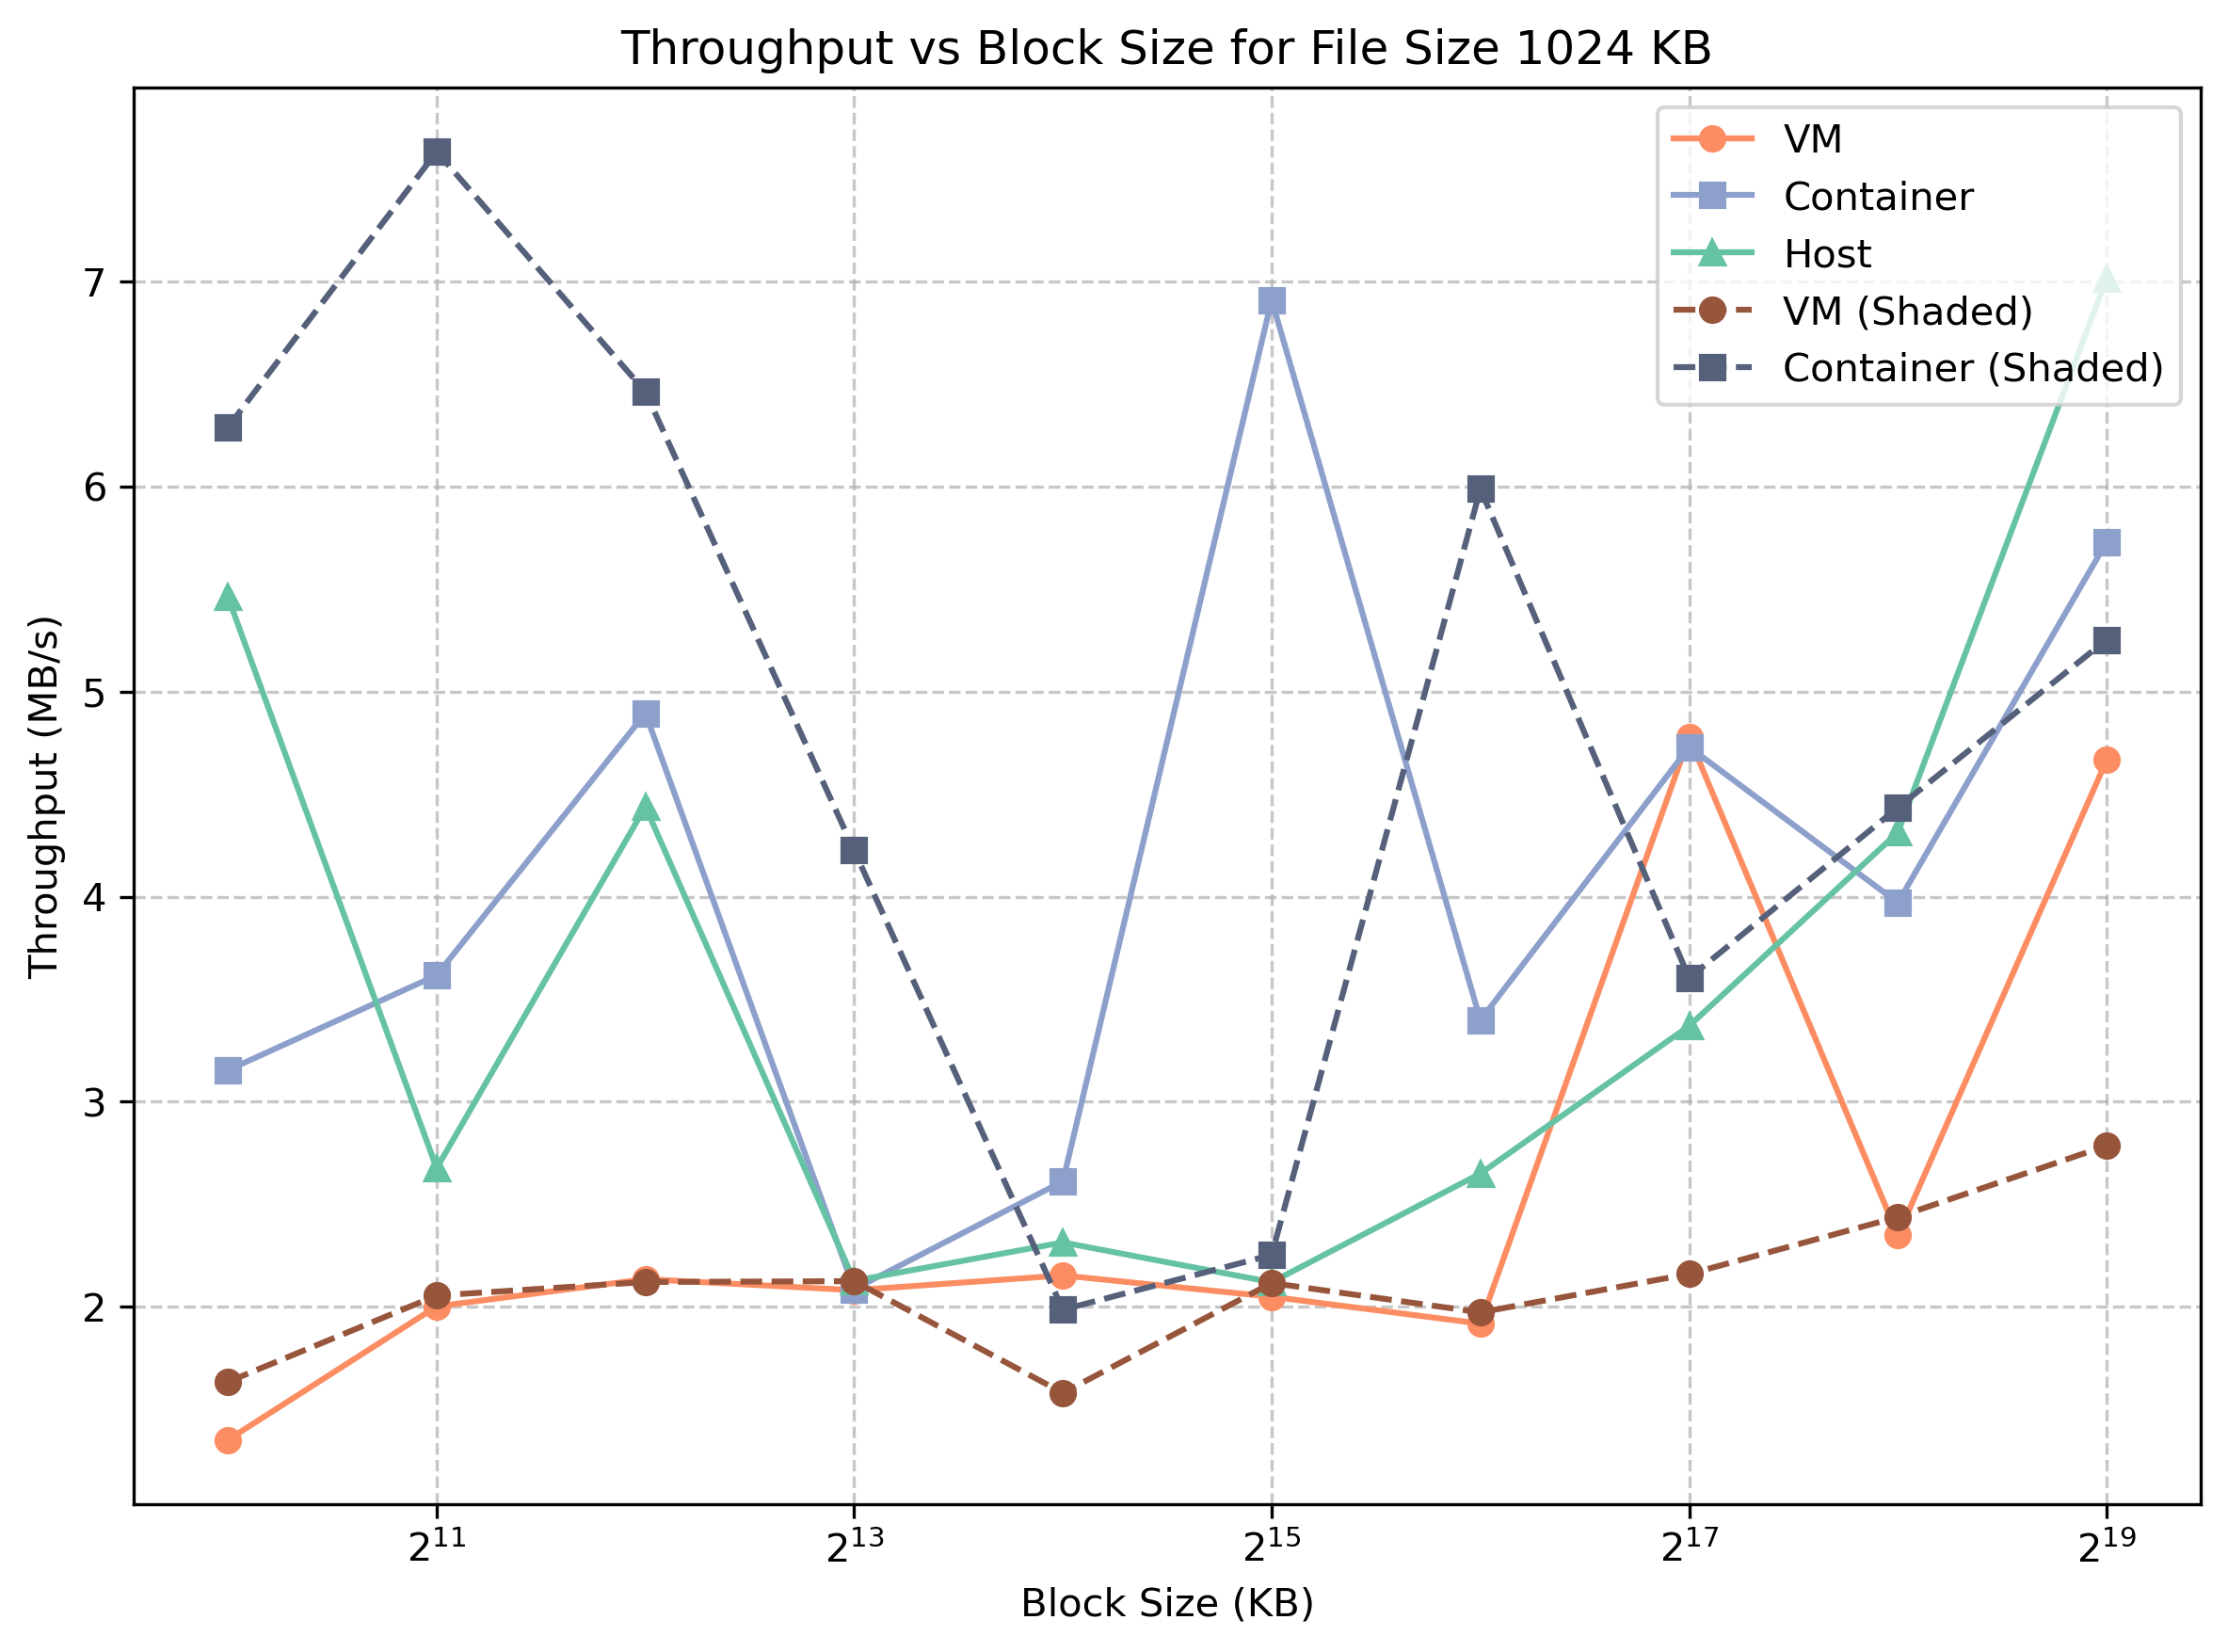
\includegraphics[width=0.8\linewidth]{assets/reader_filesize_1024.png}
    \caption{Iozone reader benchmark for a fixed file size of 1024 MB. The throughput is reported in MB/s.}
    \label{fig:reader_filesize_1024}
\end{figure}

\begin{figure}
    \centering
    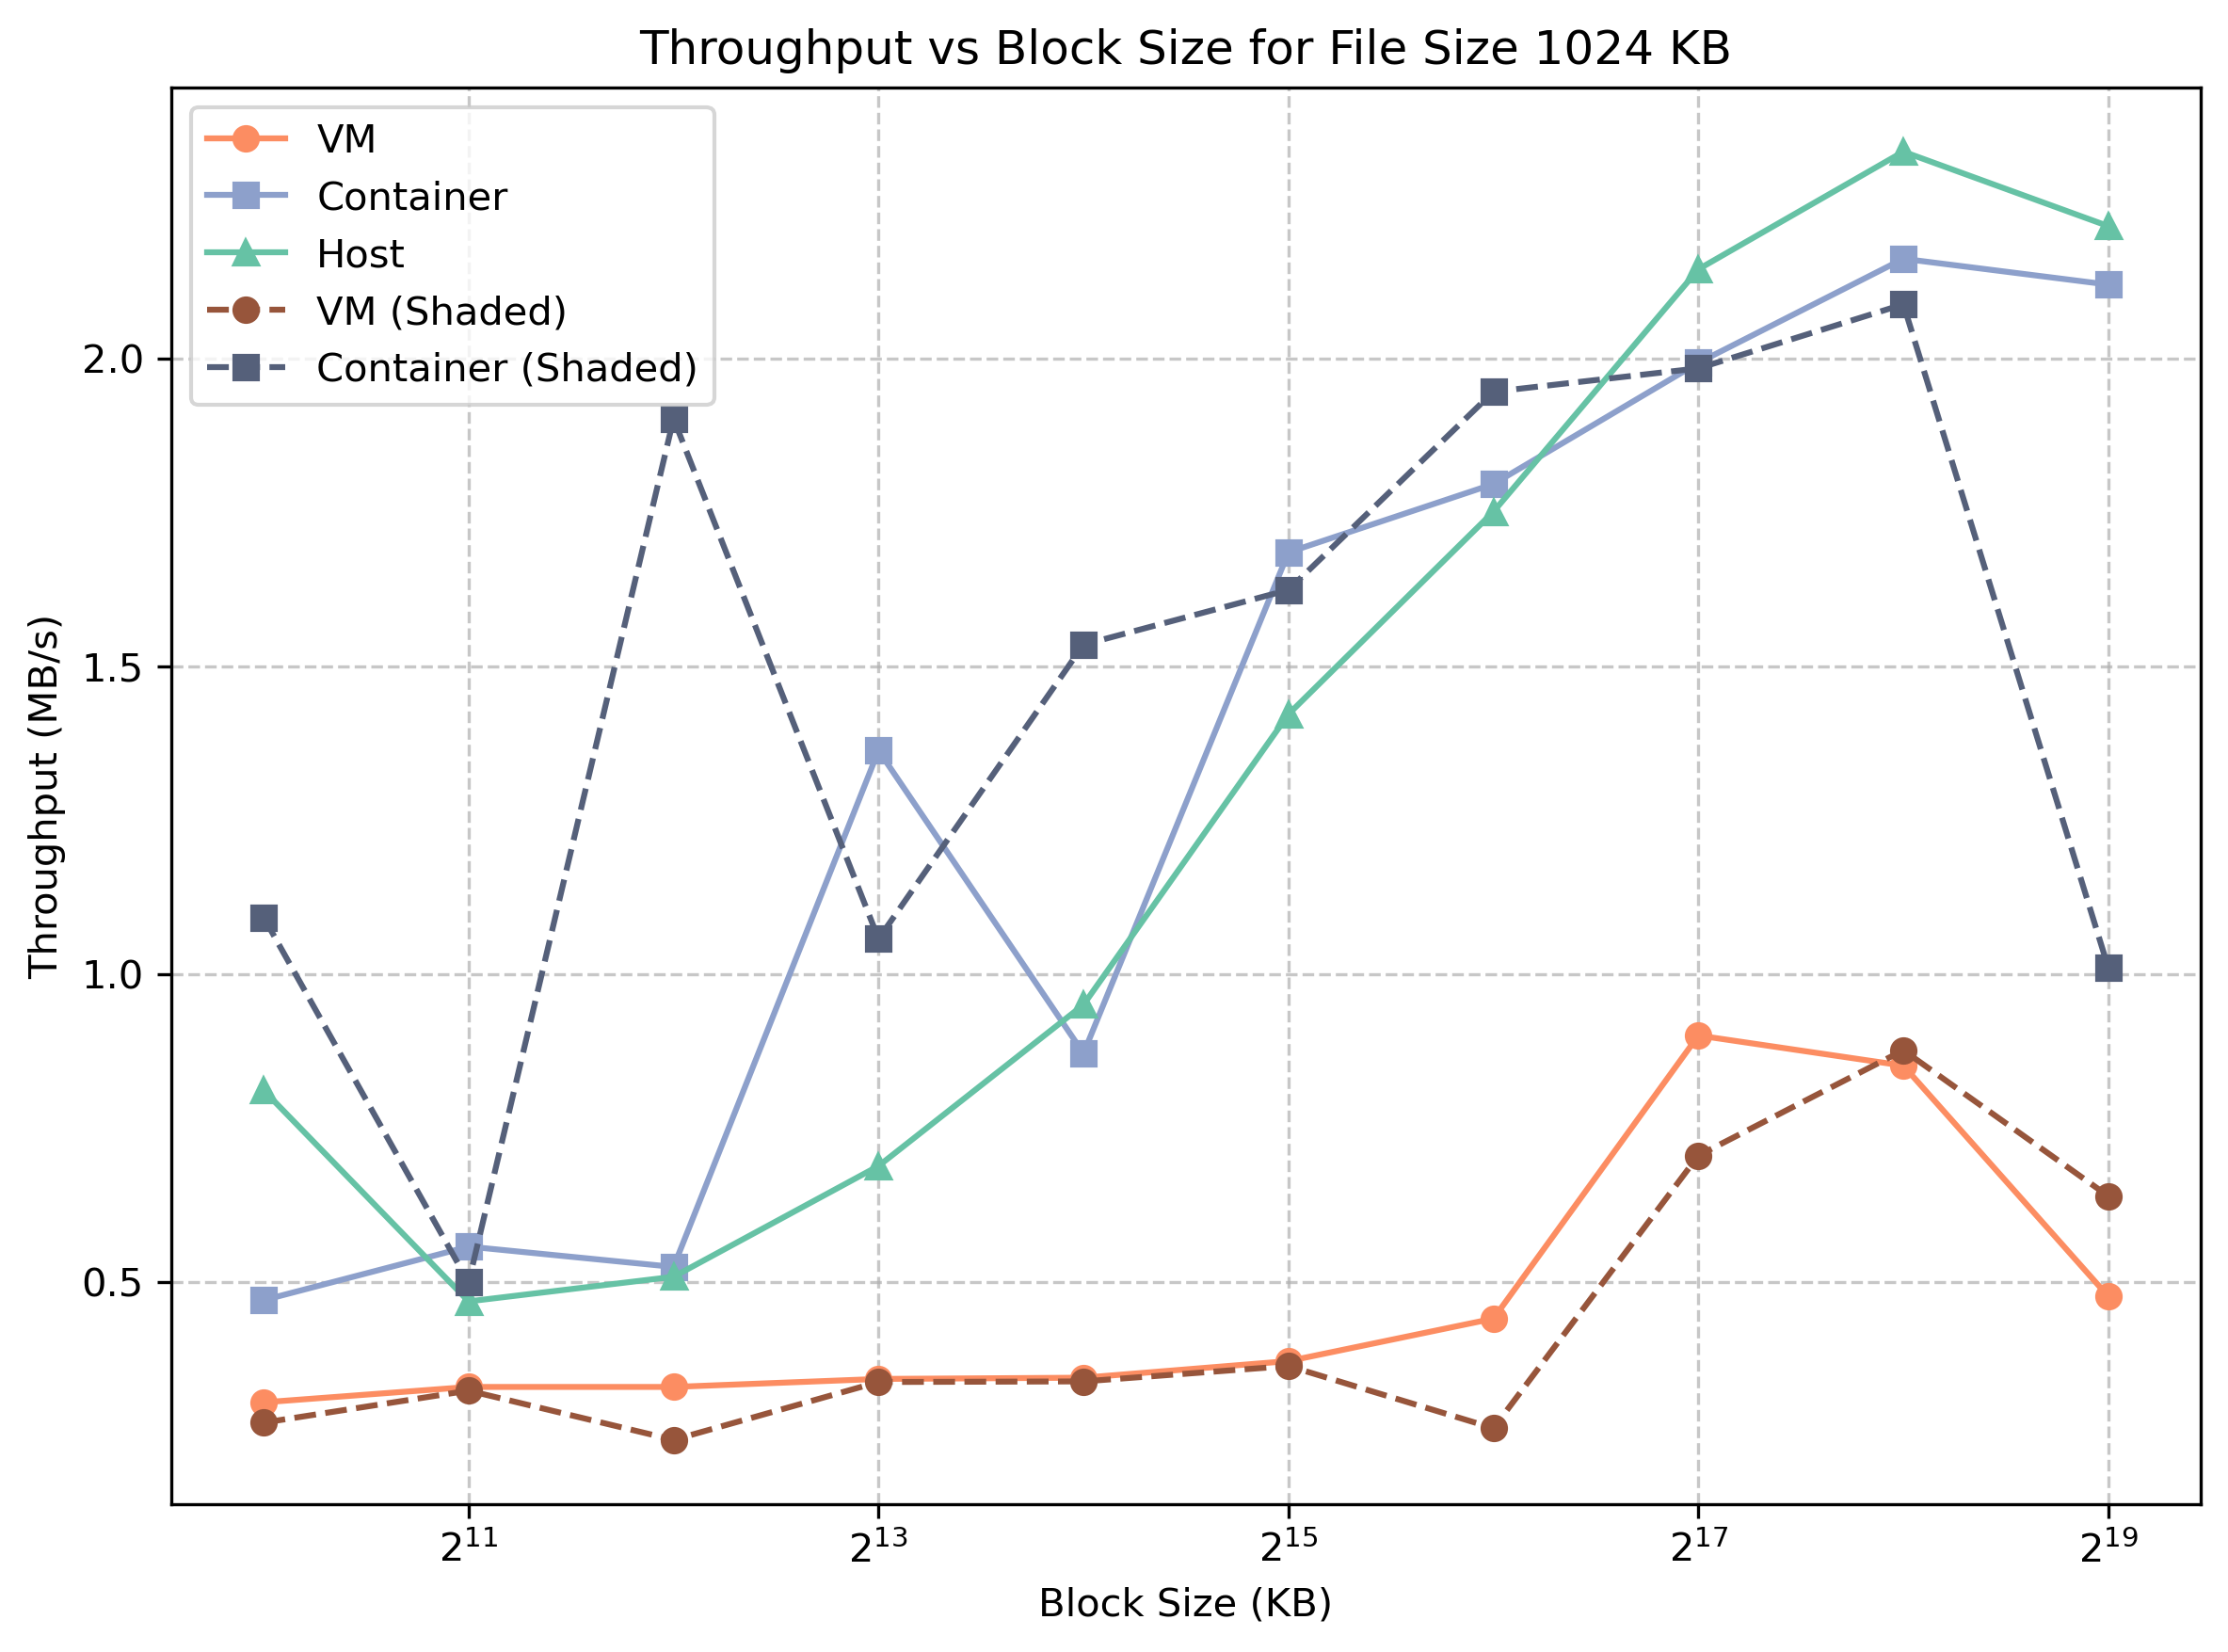
\includegraphics[width=0.8\linewidth]{assets/writer_filesize_1024.png}
    \caption{Iozone writer benchmark for a fixed file size of 1024 MB. The throughput is reported in MB/s.}
    \label{fig:writer_filesize_1024}
\end{figure}

\begin{figure}
    \centering
    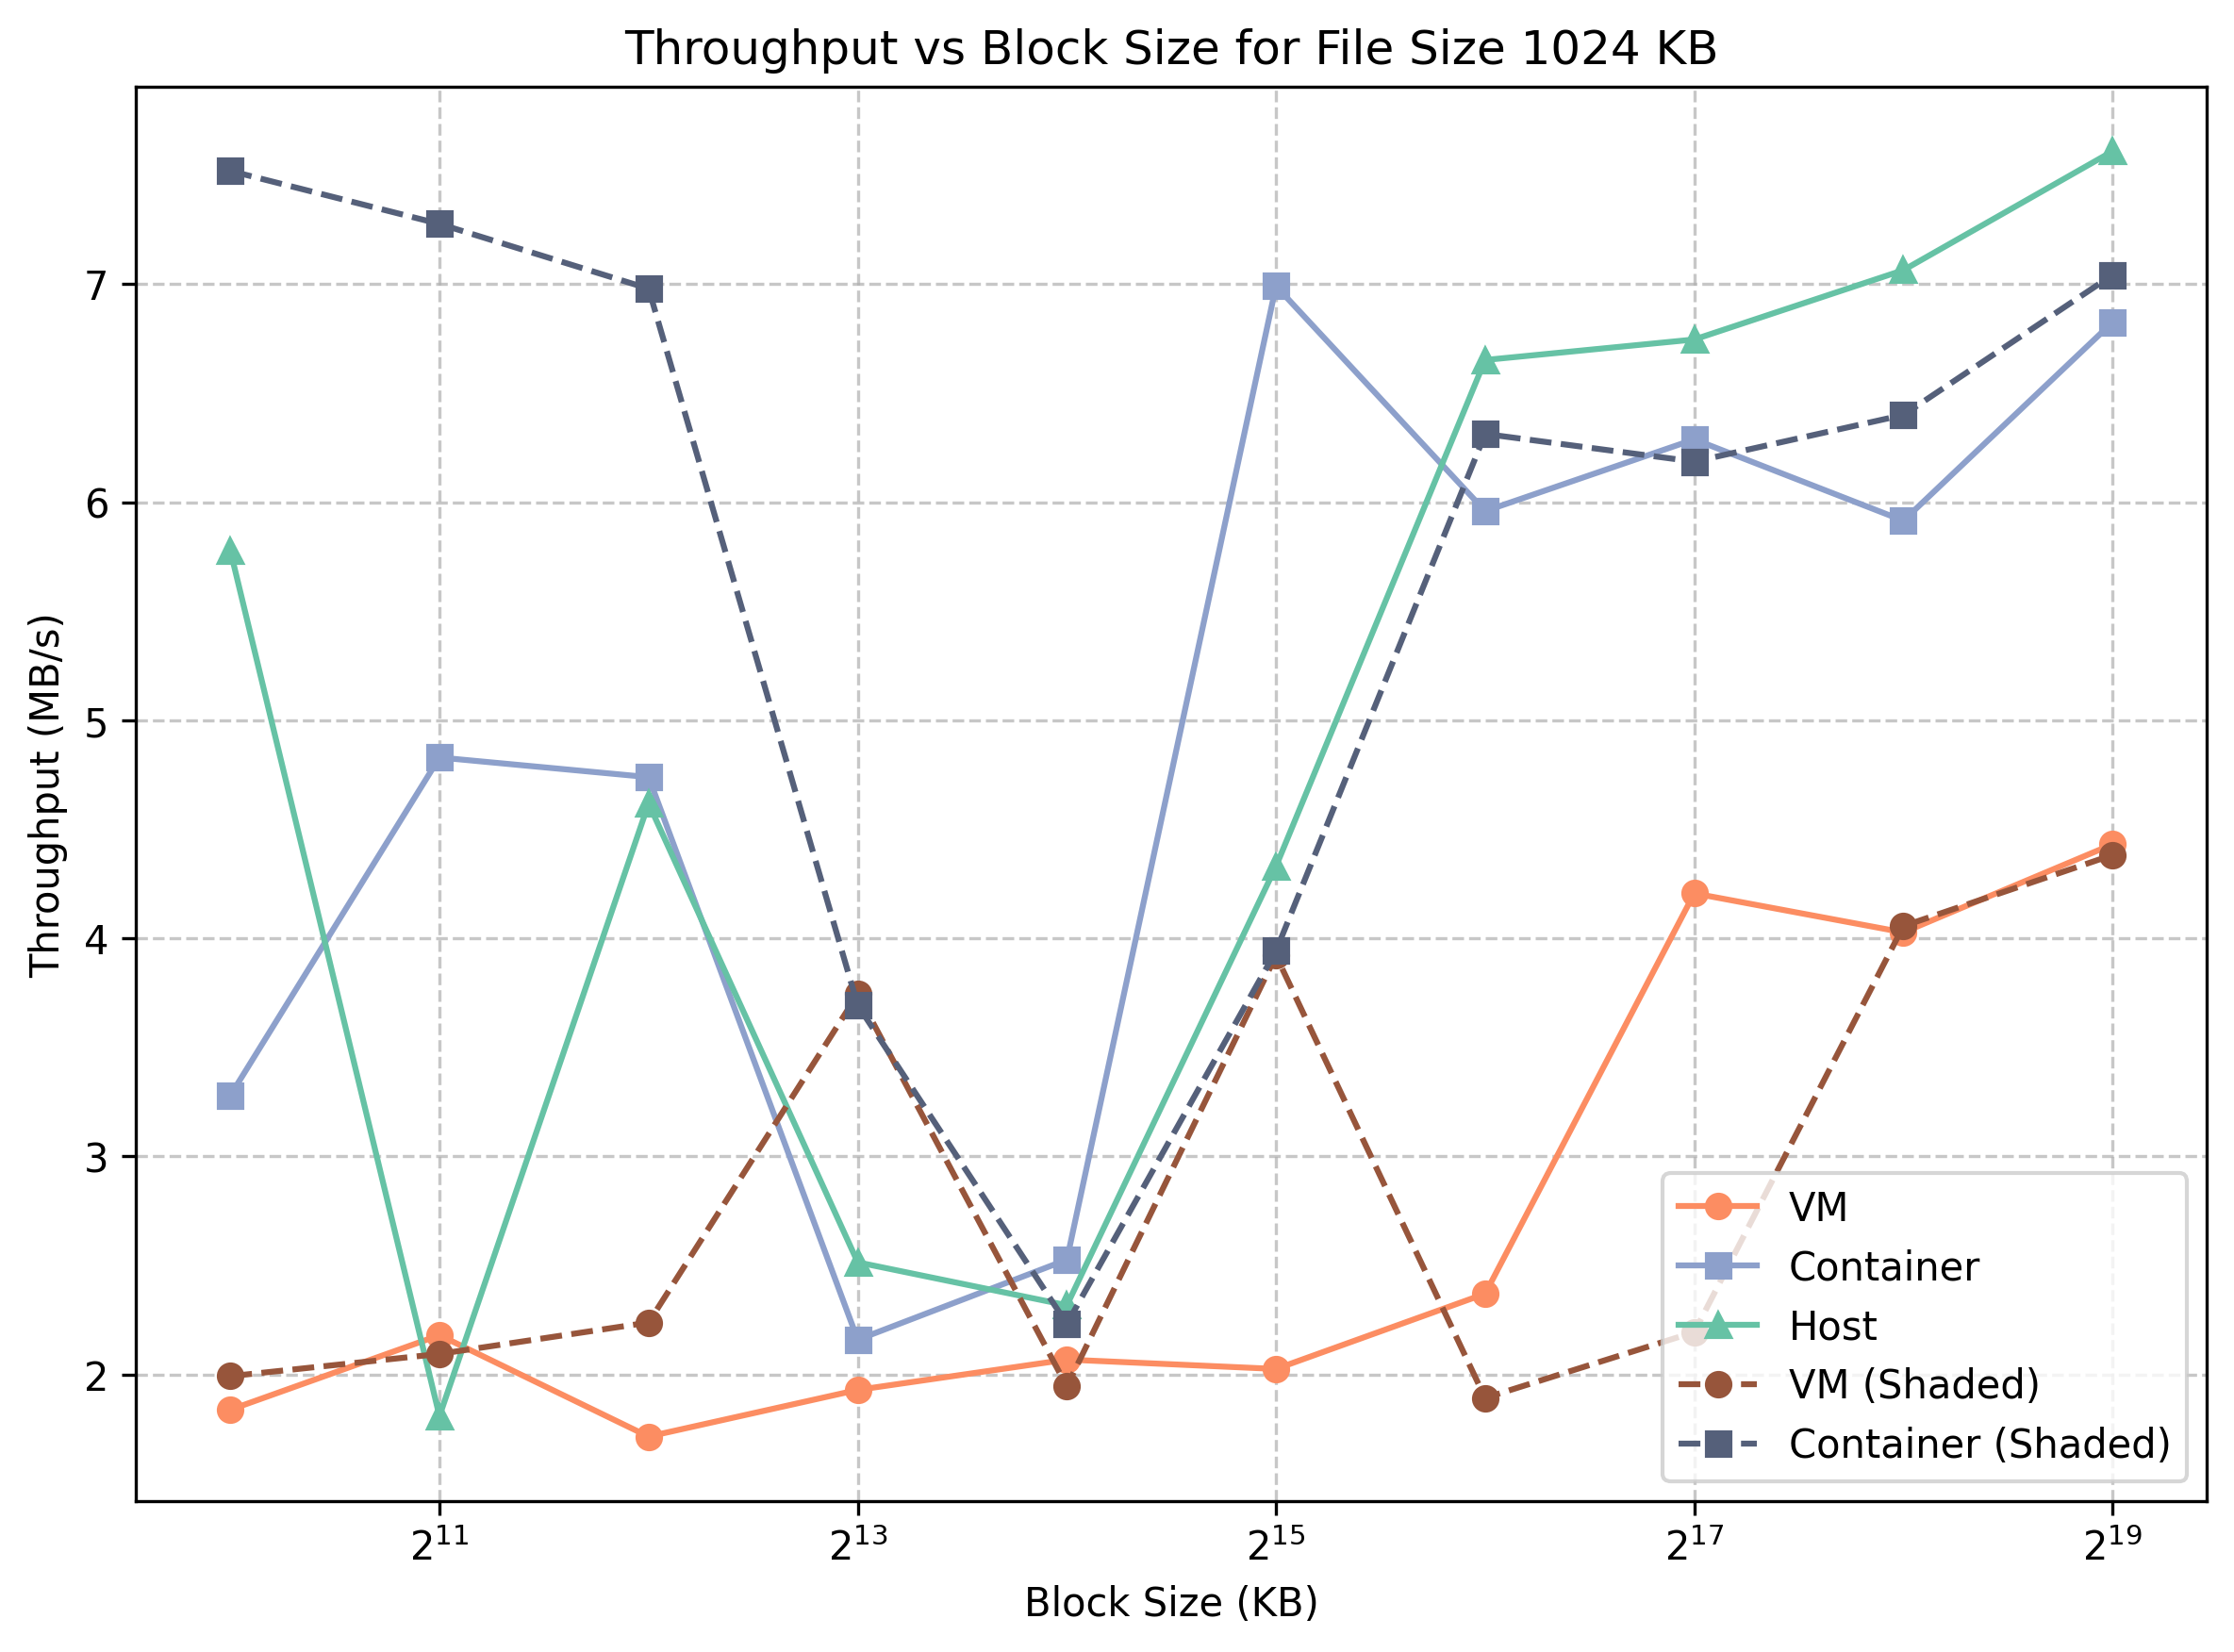
\includegraphics[width=0.8\linewidth]{assets/random read_filesize_1024.png}
    \caption{Iozone random read benchmark for a fixed file size of 1024 MB. The throughput is reported in MB/s.}
    \label{fig:random_read_filesize_1024}
\end{figure}

\begin{figure}
    \centering
    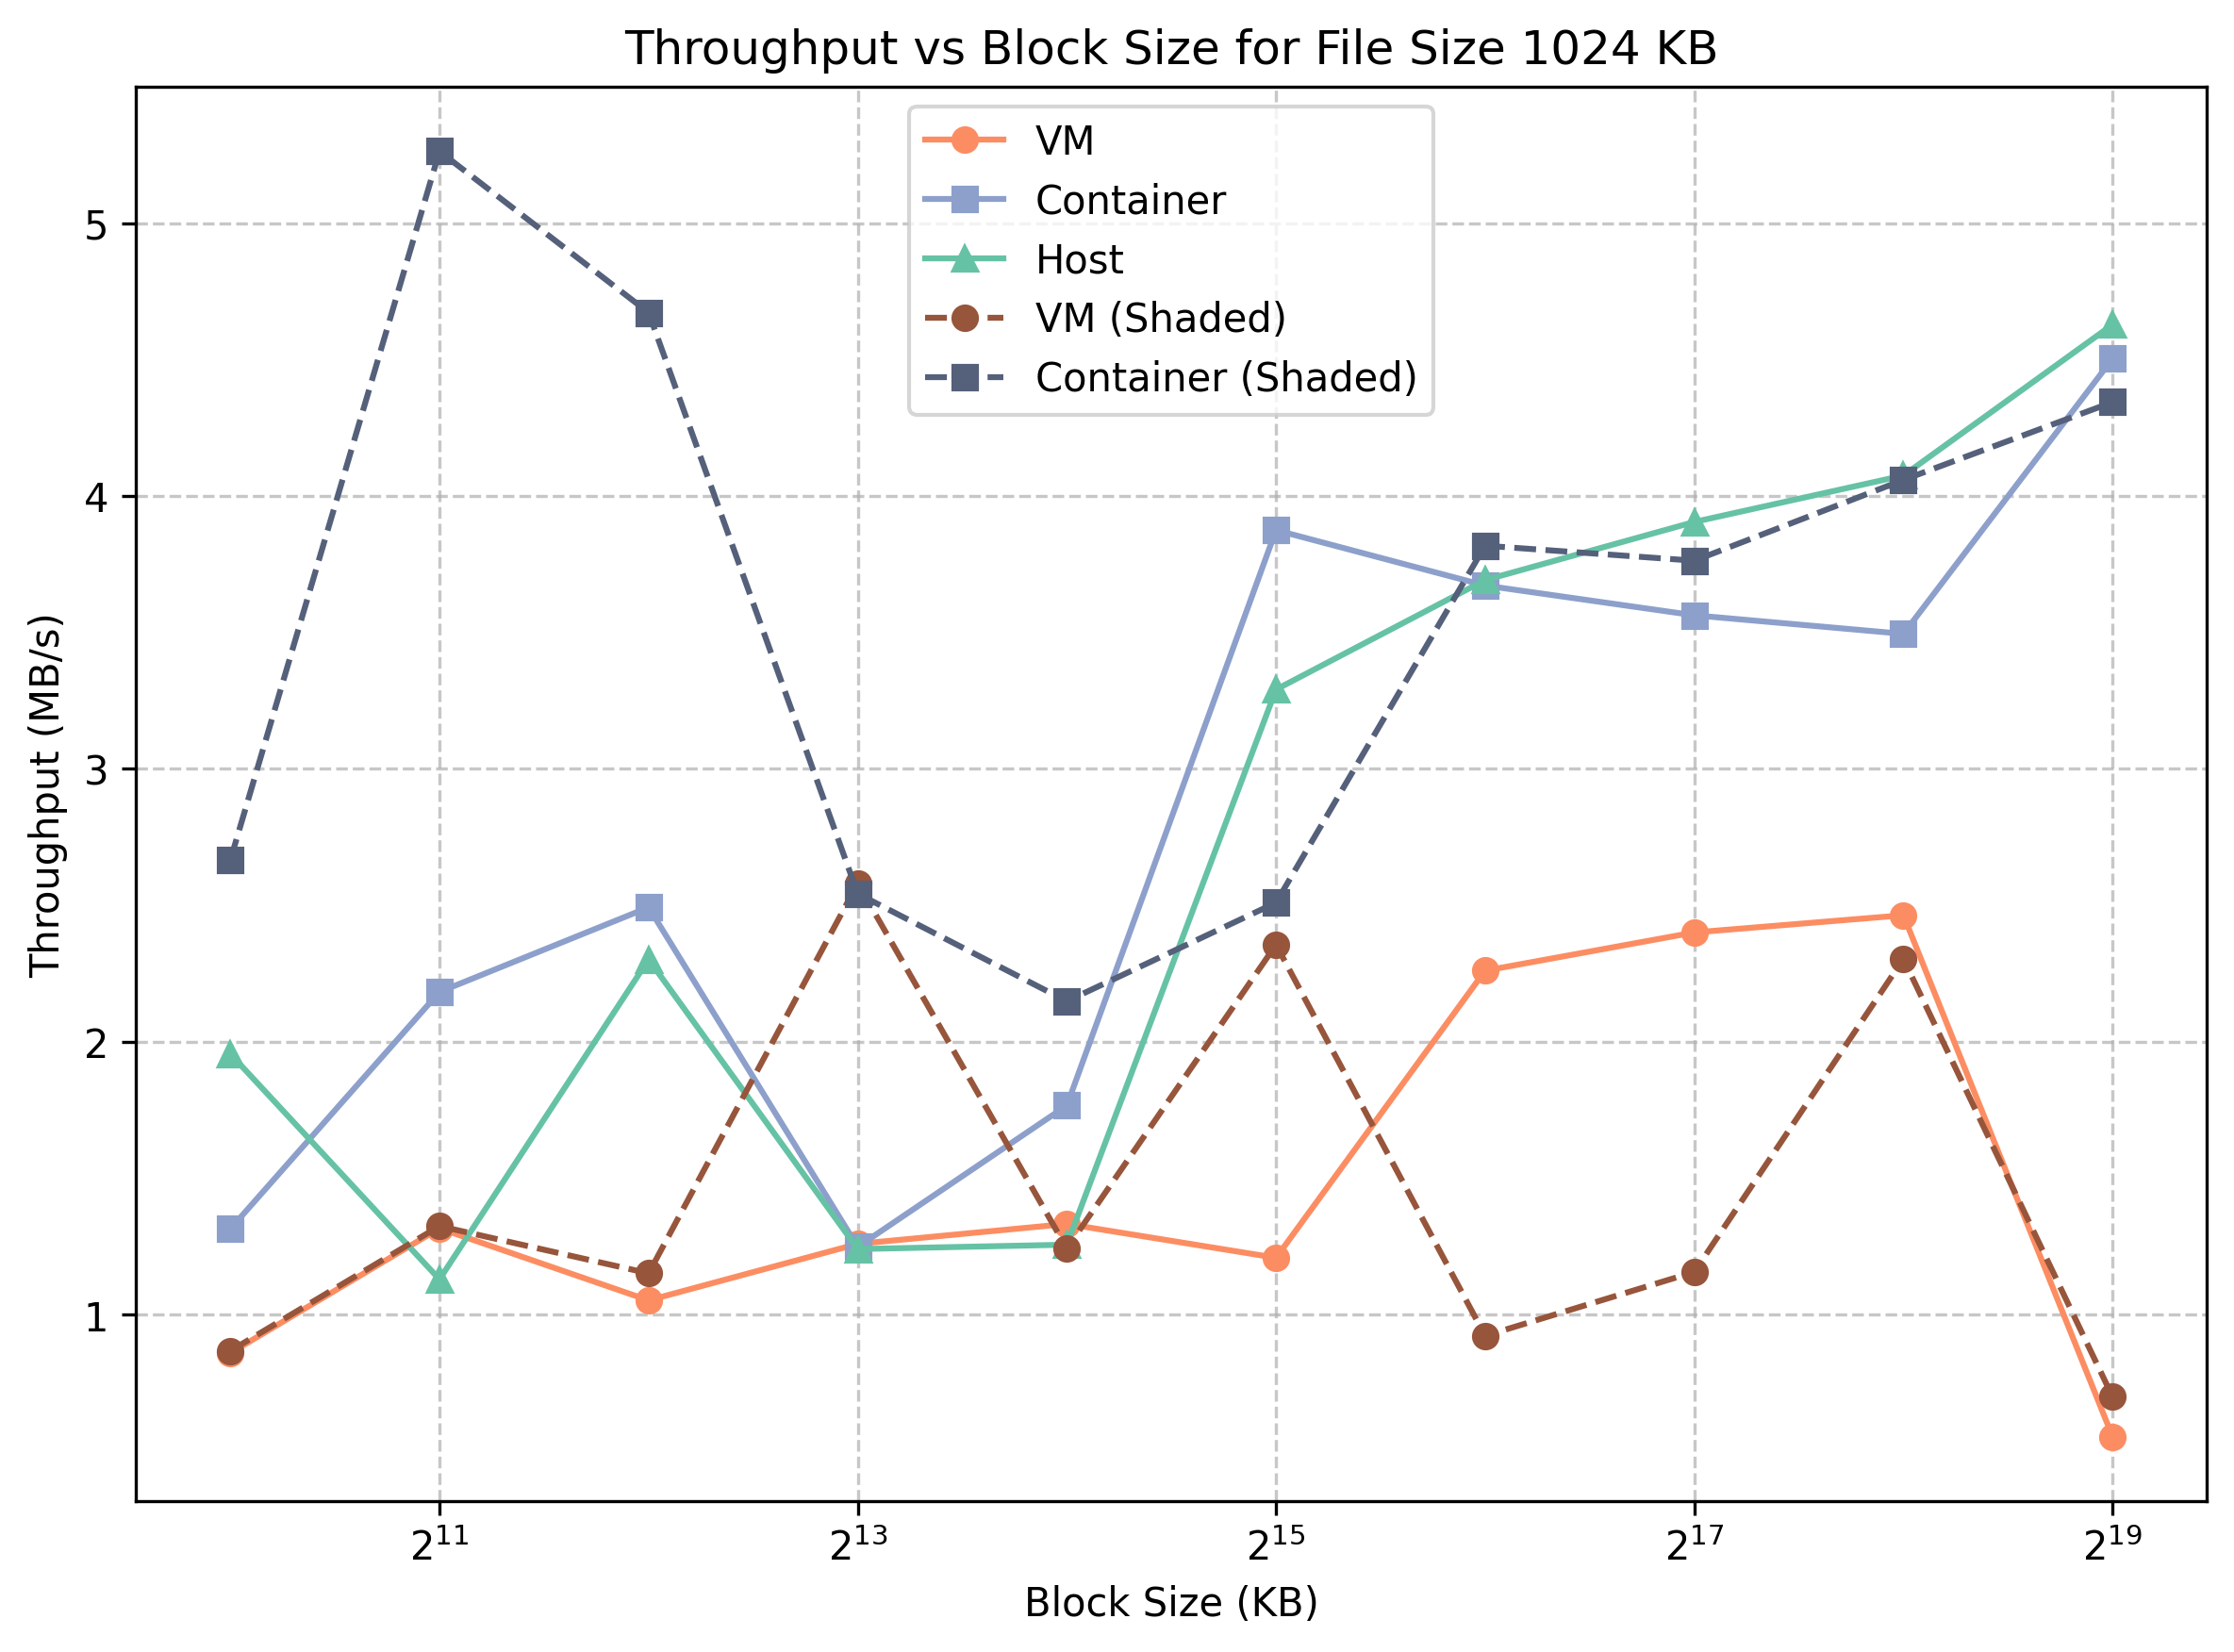
\includegraphics[width=0.8\linewidth]{assets/random write_filesize_1024.png}
    \caption{Iozone random write benchmark for a fixed file size of 1024 MB. The throughput is reported in MB/s.}
    \label{fig:random_write_filesize_1024}
\end{figure}

\subsection{iperf}

Iperf results provide a direct assessment of the network connection quality between nodes in a virtual machine (VM) cluster and those in a Docker container cluster. The Transmission Control Protocol (TCP) benchmarks reveal significantly higher bandwidth in the containerized environment, with both upload and download speeds averaging approximately $42-43$ Gb/s. In contrast, the VirtualBox-based VM network achieves substantially lower TCP bandwidth, averaging only $2.7-2.8$ Gb/s for both directions. This indicates that the TCP network performance in the container environment is roughly 15 to 16 times greater than that of the VM environment.

For User Datagram Protocol (UDP) traffic, the successfully received bitrate further underscores the superior performance of the container network, reaching 1.61 Gb/s compared to just 0.44 Gb/s in the VM setup. A critical distinction emerges in the packet loss metrics: the VM network exhibits a high average packet loss rate of 15.85\%, meaning that over 15\% of UDP packets are dropped even at the relatively modest bitrate of 0.44 Gb/s. Furthermore, the packet loss standard deviation of ±15.99\% indicates highly unstable UDP delivery within the VM cluster. Conversely, the container network maintains an exceptionally low packet loss rate of 0.01\% at the higher 1.61 Gb/s bitrate, reflecting far more reliable performance.

As observed for the \texttt{hpcc} benchmark, the stark contrast in network throughput is a decisive factor in the superior performance of container-based clusters for distributed workloads, such as StarSTREAM or the Message Passing Interface (MPI) components of the HPCC benchmark suite. The constrained network speed and instability in the VM environment inherently limit data transfer rates between nodes, regardless of CPU processing power or local memory performance. Therefore, the network inefficiencies in the VM configuration significantly hinder the execution of communication-intensive parallel applications.
\begin{table}[htbp]
    \centering
    \begin{tabular}{lcc}
    \toprule
    \textbf{Benchmark} & \textbf{VM} & \textbf{Container} \\
    \midrule
    \textbf{TCP upload} & & \\
    Bitrate (Gb/s) & $2.66 \pm 0.56$ & $42.48 \pm 6.75$ \\
    Transfer (GB) & $0.30 \pm 0.10$ & $4.91 \pm 1.11$ \\
    \midrule
    \textbf{TCP download} & & \\
    Bitrate (Gb/s) & $2.84 \pm 1.28$ & $43.04 \pm 1.66$ \\
    Transfer (GB) & $0.30 \pm 0.10$ & $4.97 \pm 0.81$ \\
    \midrule
    \textbf{UDP} & & \\
    Bitrate (Gb/s) & $0.44 \pm 0.19$ & $1.61 \pm 0.31$ \\
    Transfer (GB) & $0.05 \pm 0.02$ & $0.18 \pm 0.06$ \\
    Lost Datagrams (\%) & $15.85 \pm 15.99$ & $0.01 \pm 0.04$ \\
    \bottomrule
    \end{tabular}
    \caption{Iperf results for VM and Container, showing TCP and UDP performance metrics. The values are reported as mean ± standard deviation, calculated over four measurements ($n = 4$).}
    \label{tab:iperf}
\end{table}